%% Template for a preprint Letter or Article for submission
%% to the journal Nature.
%% Written by Peter Czoschke, 26 February 2004
%%

\documentclass{aastex62}

%% make sure you have the nature.cls and naturemag.bst files where
%% LaTeX can find them
\usepackage{graphicx}	% Including figure files
\usepackage{amsmath}	% Advanced maths commands
\usepackage{amssymb}	% Extra maths symbols
%\usepackage{natbib}

\usepackage{hyperref}
\usepackage{url}
\usepackage{microtype}
\usepackage{rotating}
\usepackage{booktabs}
\usepackage{threeparttable}
\usepackage{tabularx}
\linespread{1.2}



%\author{Daniela Huppenkothen$^{1,2,3}$, Anthony Arendt$^{4,5}$, David W. Hogg$^{2,1,6,7}$, Karthik Ram$^8$, Jake VanderPlas$^5$, and Ariel Rokem$^5$}


%\makeatletter
%\let\saved@includegraphics\includegraphics
%\AtBeginDocument{\let\includegraphics\saved@includegraphics}
%\renewenvironment*{figure}{\@float{figure}}{\end@float}
%\makeatother

%\renewcommand*\thesection{\arabic{section}}
%\renewcommand*\thesubsection{\arabic{subsection}}

\setcounter{tocdepth}{3}

\begin{document}

\title{Supplementary material for "Hack Weeks as a model for Data Science Education and Collaboration"}

%% Notice placement of commas and superscripts and use of &
%% in the author list

\author{Daniela Huppenkothen}
\altaffiliation{dhuppenk@uw.edu}
\affiliation{DIRAC Institute, Department of Astronomy, University of Washington, 3910 15th Ave NE, Seattle, WA 98195, USA}
\affiliation{Center for Data Science, New York University, 65 5th Avenue, 7th Floor, New York, NY 10003, USA}
\affiliation{Center for Cosmology and Particle Physics, New York University, 726 Broadway, 10th Floor, New York, NY 10003, USA}
\nocollaboration

\author{Anthony Arendt}
\affiliation{Polar Science Center/Applied Physics Laboratory, University of Washington, 1013 NE 40th Street, Box 355640, Seattle, WA 98105-6698}
\affiliation{The University of Washington eScience Institute, The WRF Data Science Studio, Physics/Astronomy Tower, 6th Floor, 3910 15th Ave NE, Campus Box 351570, University of Washington, Seattle, WA 98105, USA}
\nocollaboration

\author{David W. Hogg}
\affiliation{Center for Cosmology and Particle Physics, New York University, 726 Broadway, 10th Floor, New York, NY 10003, USA}
\affiliation{Center for Data Science, New York University, 65 5th Avenue, 7th Floor, New York, NY 10003, USA}
\affiliation{Max-Planck-Institut f\"ur Astronomie, K\"onigstuhl 17, D-69117 Heidelberg}
\affiliation{Center for Computational Astrophysics, Flatiron Institute, 162 5th Ave, New York, NY 10010, USA}
\nocollaboration

\author{Karthik Ram}
\affiliation{Berkeley Institute for Data Science \& Berkeley Initiative in Global Change Biology, University of California, Berkeley,  Berkeley CA 94720}
\nocollaboration

\author{Jake VanderPlas}
\affiliation{The University of Washington eScience Institute, The WRF Data Science Studio, Physics/Astronomy Tower, 6th Floor, 3910 15th Ave NE, Campus Box 351570, University of Washington, Seattle, WA 98105, USA}
\nocollaboration

\author{Ariel Rokem}
\affiliation{The University of Washington eScience Institute, The WRF Data Science Studio, Physics/Astronomy Tower, 6th Floor, 3910 15th Ave NE, Campus Box 351570, University of Washington, Seattle, WA 98105, USA}
\nocollaboration

%\maketitle

%\begin{affiliations}
%\item{Center for Data Science, New York University, 65 5th Avenue, 7th Floor, New York, NY 10003, USA}
%\item{Center for Cosmology and Particle Physics, New York University, 726 Broadway, 10th Floor, New York, NY 10003, USA}
%\item{DIRAC Institute, Department of Astronomy, University of Washington, 3910 15th Ave NE, Seattle, WA 98195, USA}
%\item{Polar Science Center/Applied Physics Laboratory, University of Washington, 1013 NE 40th Street, Box 355640, Seattle, WA 98105-6698}
%\item{The University of Washington eScience Institute, The WRF Data Science Studio, Physics/Astronomy Tower, 6th Floor, 3910 15th Ave NE, Campus Box 351570, University of Washington, Seattle, WA %98105, USA}
%\item{Max-Planck-Institut f\"ur Astronomie, K\"onigstuhl 17, D-69117 Heidelberg}
%\item{Center for Computational Astrophysics, Flatiron Institute, 162 5th Ave, New York, NY 10010, USA}
%\item{Berkeley Institute for Data Science \& Berkeley Initiative in Global Change Biology, University of California, Berkeley,  Berkeley CA 94720}
%\end{affiliations}

\newpage

\tableofcontents

\newpage

\noindent While the main text of this paper remains fairly theoretical, we aim to lay out more practical advice regarding the organization of a hack week in this supplement. 



\section{What to do before}

\subsection{Obtaining permission for tracking and studying participants}
A secondary goal of most of our previous events was to study the development of a hack week, to observe participant behavior, and quantify the achievement of learning outcomes. To this end, we invited social scientists, interested in mechanisms of scientific collaboration and educational design process, to observe our activities. These scientists then reviewed their observations and gave valuable feedback about the hack week outcomes. In order to be able to track and study participants, approval from an Internal Review Board is required. This should be done as early as possible, and having assistance from researchers in the social sciences is invaluable, in particular for hack weeks in fields that generally do not involve human subject research. Ideally, participants should consent to be contacted at the application stage, which opens up the potential of tracking both participants and non-participants and allows for evaluation of the hack week.

\subsection{Determining your objectives}

Unlike traditional conferences, where the programme is primarily driven by speaker selection, careful goal planning is essential for a successful hack week. The stated goals will continue to determine almost all of the remaining organizational questions, including space, participant selection and workshop evaluation. Is the target audience primarily students, or mature researchers, or a mix of both? Should the taught component dominate over project work or should it be only a minor programme point? Is the community to be invited more software-focused or should outcomes skew towards publishable results? Does the hack week aim to maximize its output by carrying best practices into universities and institutions that may be particularly underrepresented? These questions, among others, should have a very clear answer before any further organization takes place.

\subsection{Hack Week Location}
When considering space, both the broader location (city and country) as well as the specifics (the room in which the workshop will occur) should receive equal consideration. The non-traditional nature of hack weeks means that some students report challenges in receiving support from their supervisor or department to attend. Thus, keeping the costs of attendance low (including travel costs, room and board, and conference fees) should be a high priority when deciding on a location. Conference centers like the Lorentz Center at the University of Leiden provide funding along with the collaborative space, but have long lead times when applying for their spaces (typically 12-18 months). The same can be true for collaborative spaces within universities and active learning environments, which tend to be popular. Therefore, the search for a location should commence no later than twelve months before the workshop, ideally much earlier.
The space itself should be large and ideally configurable, with moveable tables and chairs, several screens or projectors, and an ample number of white-/chalkboards. A useful guiding principle is to book a space that fits a group at least 25\% larger than that envisioned for the workshop, and the less configurable the space, the larger the extra room should be.
There is a natural tension between keeping the group together and providing physically separated break-out spaces. On the one hand, conducting the workshop in a single large venue improves group cohesion and prevents self-segregation of researchers and ideas. On the other hand, the interactive nature of the workshop may lead to an environment where it is difficult for individuals to focus on the highly complex tasks that are typical for hack week projects. It may hence be advisable to allow for diffusion of the group into adjacent rooms, while providing ample venue for the entire group to congregate for tutorials, breaks and reports.
There should be plenty of power outlets for participants to plug in their computers.
The space should have ready access to wifi, for activities that require an internet connection (e.g., collaborative software development), and organizers should arrange in advance to provide access to visitors from other institutions.
Accessibility should be taken into consideration: is the space accessible for participants who use wheel-chairs? Are accessible restrooms available?

\section{Event Size and Duration}

Event size (i.e. the number of attendees) and event duration are important to consider during the design and planning phase of a hack week. All hack weeks we have organized so far have had group sizes between 40-60 participants. The number of attendees resulted from a number of different design considerations. One practical consideration was the size of the available location: especially the project-focused parts of a hack week generally require a reconfigurable space with more seats than attendees, such that spontaneous organization in sub-groups is easy. However, group size is also important in the context of community building, group dynamics and programme decisions. We limited group size to a maximum of 70 participants, because previous anecdotal evidence has shown us that this is about the maximum group size where interactions between all participants is still possible. We wanted to ensure that all participants had an opportunity to at least meet all other participants, in order to facilitate community building and keep the group from fracturing into cliques. Another important consideration is representation along the many axes of diversity we considered. For example, whereas a single undergraduate participant might feel like an outsider, admitting three or four can mitigate alienation. Similarly, in order to foster active collaboration among many different subfields, we endeavored to admit participants with many different types of overlapping expertise. Having a set of participants that is too small could interfere both with these goals of representation and of fostering interdisciplinary collaborations and networking. Smaller groups (of less than $\sim$30 participants or so) will need to attend to participant selection particularly carefully in order to achieve the desired level of diversity across participants. 

All hack weeks organized by us up to now have been five days. This duration was chosen to allow enough time for both learning and project work at the same time. Participants often arrived with ambitious project ideas, or with the goal of taking newly learned methods and applying them to their data sets right away. Thus many projects tended to extend over multiple days. Attendees who participated in multiple projects often used the hack week to try out several different ideas. A five-day hack week allows for ample time for these ambitious projects or experimentation, where a shorter hack week would necessarily have to be more constrained and focused. At the same time, hack weeks tend to be exhausting. Project work often extends into the evenings, and requires prolonged phases of high concentration of participants, thus we limited our hack weeks to five days in order to avoid excessive fatigue among our attendees.

It is worth noting, however, that these guidelines were developed out of design considerations rather than experimentation and testing. In the future, we plan to experiment with the format, duration and size of these events and continue to evaluate their interplay with our objectives.

\subsection{Participant selection}

As we lay out in the main text, participant selection is one of the most important design decisions as part of a hack week. Conversations about participant selection, and planning of selection strategies should commence early, ideally at the start of the organizing process.
Because selection procedures are subject to a whole range of human biases, it is worth thinking critically about established procedures and how to improve them. At the same time, hack weeks are comparatively lower-stakes events than other situations where cohort selection is relevant, like e.g.\ graduate school admissions, thus hack weeks may also serve as test beds for experimentation and improvements that can inform selection in other contexts.

The hack weeks presented here used different approaches, that nevertheless share several common themes and ideas. In particular, they focus on making the selection procedure as quantitative as possible and use the data collected during each stage of the process to critically evaluate the efficacy of the process and its subject to human bias.
Secondly, much energy is expended early on in the design of the application form, which often use a combination of open-answer and multiple-choice questions to assess candidates' suitability, skill levels and backgrounds. Care must be taken when designing questions assessing skill levels, because options such as ``beginner'' or ``expert'' have no absolute scaling and may have different meanings to different applicants. They may also be subject to intrinsic biases, if candidates of certain backgrounds systematically underestimate or overestimate their skill levels compared to other candidates (the Dunning Kruger effect). It is thus advisable to calibrate skill levels on concrete milestones. For example, instead of asking participants whether they are ``beginners'' or ``experts'' at machine learning, we instead asked them whether they had done machine learning for class work, had used techniques from machine learning in their own research, or had developed and implemented their own methods. Similarly, questions about programming skills may ask whether participants can perform a particular task in one of a list of languages (e.g., ``write a module or a library'').
Responding to questions about demographic characteristics should generally be optional, and organizers should consider how these questions might interact adversely with workshop goals, e.g.\ via stereotype threat. For example, Astro Hack Week only asked whether an applicant considered themselves a minority with respect to gender identity within astronomy, rather than asking them to explicitly self-identify within a specific category. Meanwhile, neuro hack week opted to ask about gender ethnicity and race, using questions that are standardly used for example, when collecting statistics about study participants.

 For any kind of merit-based selection, committees should critically examine their assumptions about reasonable expectations regarding (minimum) skill levels required for participation. Candidates from underrepresented groups, smaller institutions or other countries may have had fewer opportunities to learn relevant skills. Consequently, in a merit-based selection based on these skills these questions may effectively trace demographic diversity and lead to biased selections even when committees are overall vigilant. If a strict merit-based selection is part of the procedure, it should be performed with these caveats in mind. It is always a good idea to check the results of any selection procedure for intrinsic biases. For example, visual comparisons of the group selected based on merit versus the group not selected with respect to various demographic variables may easily reveal unintended biases introduced at this stage, and the procedure can be adjusted and refined.
 
Since human decision makers also routinely overestimate their ability to forecast future performance of a candidate and underestimate intrinsic variance during selection procedures, ~\cite{highhouse2008} it may be beneficial to set a fairly tolerant threshold for acceptance based on merit criteria, and select the cohort from this meritous pool via e.g.\ via an algorithm, imposing outside constraints on the selection based on the goals of the workshop. 

One solution to the latter problem is implemented in the software \textit{entrofy}\footnote{\url{http://github.com/dhuppenkothen/entrofy}}). 
The algorithm aims to find a group of participants that together match as closely as possible a requested distribution on specified dimensions (e.g., career stage, geographic location, etc.), to meet pre-set fractions set by the organizers.
It is worth noting that this algorithm is vulnerable toward biases in two ways: firstly, humans will set the target fractions for any category of interest.  
Any human biases involved in setting these target fractions will be perpetuated in the selection procedure. 
Secondly, perhaps more obviously, the algorithm can only act on information that has been collected.
Biased participant sets may still result from selection procedures that fail to include crucial categories. 

The overall selection procedure for Astro Hack Week comprised a two-step process. In the initial step, we performed a blind assessment for suitability using open-ended questions querying candidates' motivations for attending the workshop, and their goals for attending. We only excluded a small fraction ($<10\%$) of applicants at this step, because our goals aligned with admitting a wide range of different skill levels and backgrounds. Applicants were generally either excluded for being an obvious mismatch with the workshop goals (as in the case of an Android developer applying to work on an unrelated game) or for being duplicate entries. We subsequently used a range of categories queried with multiple-choice questions  on the application to maximize diversity across these categories, which included career stage, gender identity, racial/ethnic identity, geographic origin, programming background, machine learning skills, statistics knowledge, and previous attendance at Astro Hack Week. Targets within each categories were set according to the different workshop goals. For example, we set ambitious goals of admitting 50\% attendees from underrepresented minorities with respect to gender, race and ethnicity with the goal of increasing representation of these groups with astronomy and data science. Similarly, we set targets for other categories (e.g. skill levels) in order to maximize goals around collaboration, networking and fostering interdisciplinary exchange of knowledge. Subsequently, we used a greedy optimization algorithm to jointly optimize over all categories simultaneously. We evaluated our results by directly comparing the characteristics of the selected set of participants with both our targets and the distribution of the set of all candidates. For demographic characteristics specifically, 42\% of participants in both 2016 and 2017 considered themselves a minority with respect to gender identity in astronomy, and 32\% of participants in 2016 (2017: 33\%) considered themselves a minority with respect to racial or ethnic identity. About half of the attendees were students ($\sim$40\% graduate students, $\sim$10\% undergraduate students), another $25\%$ postdoctoral fellow, and the remainder about equally split between research staff, tenured and tenure-track faculty, and participants in non-academic careers.

Neuro hack week took a different approach: participants provided CV as part of their application, in addition to answering questions about their technical and research background, and writing a short statement of the purpose of their participation. Each application was reviewed by several instructors using 1-10 scales on several criteria: technical and computing experience, research experience, the quality of the statement, an assessment of the contribution of participation to the applicant's career, and an assessment of the degree to which participation would increase the representation of groups that are usually under-represented in neuroscience and computing. The scores were combined, applicants were ranked according to the combined score, and the 40 highest-scoring applicants were then selected to participate. As an example,  this procedure resulted in gender parity in 2016 and near-parity (17 women and 23 men) in 2017. In neuro hack week as well about half of the participants were students (though no undergraduate students participated), about $25\%$ were post-docs, with the remainder including research staff and faculty members.

\subsection{Funding}

We have worked to minimize the cost of registration for our events in order to enable broad participation, especially for participants from institutions, countries and demographics that are generally underrepresented at other meetings. Locations that offer some funding or provide free space are preferable to those that do not.
We have found that travel grants are of crucial importance especially to undergraduates, students from minority backgrounds and participants from underrepresented countries. We found that minority participants disproportionally decline to attend, and often cite lack of sufficient travel funding as the primary reason. In particular if increasing diversity in the more technical aspects of a field is one of the workshop's goals, providing enough travel funding for between five to ten participants can make a significant difference in allowing minority researchers to attend.
Funding for some activities can be obtained through commercial vendors.
For example, cloud computing providers have educational programs that provide cloud computing credits for students.
Other corporate sponsorships of certain activities or of the event as a whole can be used to lower participation costs, and make participation more feasible for many participants.
Federal funding agencies are also sometimes able to fund hack weeks and similar activities under traditional funding mechanisms that support training. For example, Neuro hack week 2017 was supported through a grant from the National Institute of Mental Health through their standard R25 training grant mechanism, and this grant continues to support it in extended format in coming years.

\subsection{Code of Conduct}

An overarching goal of every hack week is to provide a welcoming, comfortable, and inclusive environment for participants to learn and work.
However, disparities in backgrounds, knowledge and experience, together with the close collaboration much of the hacking requires, creates the potential for conduct that might offend participants, and preclude them from participating fully.
For this reason, a hack week should have a clear and enforceable code of conduct, that can guide the behavior of participants, and help organizers maintain a professional and welcoming environment.
It is the responsibility of the organizing committee to discuss what belongs in the code of conduct, how it should be enforced, and prepare for different scenarios and their possible resolution in advance.
A part of this could and should be the recognition that participants (and, indeed, members of the organizing committee) may occasionally violate the code of conduct in minor ways, and allow for tools and mechanisms to resolve these infractions. Major infractions, conversely, should be taken seriously and in severe cases lead to exclusion of participants.
Aside from important provisions banning discrimination on the basis of demographic characteristics, there may be domain- or workshop-specific clauses that may require recognition. For example, as communities move between programming languages or techniques, shaming participants for their choice of method or language should be strongly discouraged, since it will make participants feel unwelcome, defensive and inhibit learning on a larger scale.
Even if no code of conduct infractions are expected, the very design of such a code sets expectations, and helps signal to participants that organizers are thoughtful of creating a welcoming environment, which in turn feeds back to the creation of such a space.

\subsection{Communicating with the Outside World}

Because hack weeks have enjoyed considerable popularity, they have often been oversubscribed. This leaves organizers with an important decision: given the necessity of turning a large fraction of applicants away, what methods does the group wish to employ in order to communicate during the hack week with the wider community not in attendance? Tutorials may be live-streamed via popular services such as youtube, but aside from the technical complexity of setting up a reliable live stream, their interactive format may not easily lend themselves to the one-directional communication of a video feed. Even so, live streams have proven to be both useful and popular in the past, but require considerable effort to set up. At the very least, there should be some method of real-time communication with the in-group. Twitter has proven itself to be an effective medium of general communication with the wider community, including hack pitches, questions during tutorials and collaboration with researchers outside of Astro Hack Week. However, the closed nature of Twitter to those with an account may not make it the ideal platform for participation. Other open-source formats that do not require sign-up, such as Matrix, may be more compatible with the hack week format \footnote{\url{https://dave.cheney.net/2017/04/11/why-slack-is-inappropriate-for-open-source-communications}}. Important documents such as programme (and especially programme changes) as well as hack descriptions should be open to the public and communicated clearly to facilitate collaborations with outside researchers.

It is, in principle, possible to organize an entire hack week virtually. However, the format rests firmly on a foundation of community-building and creating opportunities for participants to exchange ideas and knowledge. While not impossible to achieve in a virtual setting, both would be significantly harder than in a single physical location, to a point where the lack of immediate exchange may severely limit to generate successful new collaborations and ideas. We thus recommend against running a purely virtual hack week.

\section{During a Hack Week}

Unlike traditional conference, where the programme is generally set by pre-selected talks, hack weeks require additional involvement from the organization committee during the hack week itself.

\subsection{Tutorials}
Tutorials provide a mechanism for rapid knowledge sharing and are often one of the most useful components of a hack week. Unlike traditional lectures, in which more time is available to explore numerous topics in depth, tutorials aim to deliver only the most essential information while ensuring students remain engaged and interactive. Moreover, the need for an instructor to balance prepared material with spontaneous, interactive learning, while attending to community building and inclusive practices, can be difficult for even the most seasoned educator. Therefore careful planning and preparation is necessary for effective delivery of a hack week tutorial. Tutorials may also be video-taped and shared with a broader community. We have found that video recordings of tutorials are rather popular, with some of them drawing more than 1,000 views.

We have experimented with numerous designs in delivering our hack week tutorials in a way that is student-centered and focused on meeting each student at their particular skill level. We have observed that, especially during long tutorials and with a particularly diverse group of students, there is a natural separation between participants who are focused on gaining new knowledge as it is being presented, versus those who already possess this knowledge and hence turn their attention to other subjects as the tutorial is ongoing. In practice, this concern can be mitigated by explicitly involving experienced participants in the tutorials. We encourage instructors to call upon experts in the audience to identify themselves and effectively act as teaching assistants. Expert participants often find this gratifying because it allows them to test their own understand and improve their skills by learning through teaching. At the same time, beginners benefit by having increased interactions with other hack week participants, thereby increasing team cohesion and building community. Another technique to engage expert participants during the tutorial is to invite them to work through more challenging content located in the online lesson, which will not be covered in the session, but for which they can obtain help during the tutorial.

Some of our hack week tutorials follow the structure of the Software Carpentry model \cite{b:wilson-swc-lessons-2016}. The content is divided in to a series of lessons, each having a well-defined set of learning objectives, key questions, and expected outcomes. Interspersed throughout each lesson are a series of exercises which participants work through at their own pace. We frequently use a method drawn from Software Carpentry whereby students indicate their need for help on an exercise via posting a colored sticky-note on their computer. This provides a simple method to deliver help to those students who need it without interrupting the flow of the tutorial. We encourage instructors to develop online material to accompany their tutorials, either in the form of Jupyter Notebooks \cite{kluyver2016jupyter} or following the markdown templates provided by Software Carpentry. This way the hack week ``curriculum'' can be built up over time and students can refer to online content after the tutorial if they need to revisit certain topics. Depending on the content, some instructors convey concepts during the tutorial via ``live-coding'' while others display static code and their results. Either way, we find dividing code into short blocks, each with a specific task, helps participants from becoming saturated with information.
In some cases, tutorials require substantial software installation and data. Though we encourage participants to install these software dependencies on their own computers, so that they can continue using them after the tutorial, this is sometime so complicated that it slows down teaching. In some cases, we have experimented with \emph{Jupyterhub}\footnote{https://jupyterhub.readthedocs.io/en/latest/} to provide students with immediate access to a computational environment that provides teaching materials (e.g., Jupyter notebooks), software dependencies, and data \cite{holdgraf2017portable}. Providing access to an ephemeral consistent environment for the purpose of teaching has become even simpler with the recent advent of the \emph{Binder} system \cite{Holdgraf2017-pd, Titus_Brown_undated-pc}.

While the short duration of the tutorial format helps us minimize the problem of information overload, it can be challenging to decide on the scope and breadth of material to be covered. In-depth collaboration among instructors in advance of the event is particularly valuable in this regard, to assess which methods or subjects will be most useful for the specific audience. We suggest that the primary goals of the tutorials should be to provide an entry point into an exploration of participants' datasets, opening the door to more thorough study outside of the hack week. Given the broad span of available tools and topics, the organizing committee should seek to teach content that represents the state-of-the-art and is deemed to be of greatest use to the broadest span of participants. A common theme across all of our hack weeks is to teach initial tutorials in version control, command line interfaces, data science platforms and practices of reproducible research. These tutorials endeavor to provide a common baseline of techniques that participants can build on in other tutorials and project work. Subsequent tutorials are then delivered in more domain-specific fields, but can be arranged in a way that builds knowledge constructively through the week. In some cases, it may be advisable to recommend some theoretical texts as reading before attending the hack week, though it is likely that speakers should not count on every participant arriving with the same knowledge baseline. Because of their practical nature, however, software requirements should be announced as early and clearly as possible, with the expectation that participants will have installed necessary software in advance. It may be helpful to designate some time early on in the meeting to trouble-shoot installations before tutorials begin in order to avoid losing significant time during the actual tutorials.

It is noteworthy that in practice, the mixed audience and interactive setting can often lead to impostor syndrome (see below) among the speakers, who lose their explicit status as expert among the participants. It is therefore imperative that speakers are made aware very early about the audience so that they can plan their tutorial accordingly. It also helps to make them aware that participants may be taking the role of teaching assistants during exercises and include them in the teaching, rather than see them as adversaries who may seek to correct them. Conversely, experts may ask pointed questions about fundamental, important concepts, both in order to help the audience gain a deeper understanding and to encourage questions, especially from junior participants, who may be hesitant to ask questions due to their own impostor syndrome. At Astro Hack Week, we encourage the organizing committee and experienced participants to ask questions, particularly when they know the answer but think the concept may not yet be clear to parts of the audience. This has in the past led to exchanges between experts that have greatly contributed to the tutorials in ways that were both unplanned and unexpected for all involved, beginners and experts alike. Including experts in the teaching also takes pressure off teachers during exercises, when demands on the speaker are generally high.

To summarize, a good tutorial will:
\begin{itemize}
\item be very clearly tailored to the audience and narrowly scoped,
\item strictly limit the amount of lecture-style teaching to less than 50\% ,
\item use experts in the audience to ask key questions and act as teaching assistants during exercises
\item communicate technical requirements at least a week before the hack week
\end{itemize}

\subsection{Break-Out Sessions}

Because instructors and organizing committees are unlikely to know in advance what projects and data sets participants will bring, often there will be topics and methods not covered in the pre-planned tutorials that are are of interest to the audience. Here, break-out sessions offer an alternative: short (30-45 minute) tutorials that are fairly spontaneously organized (with as little a lead time of a few hours) and often taught by expert participants in the audience. These tutorials can be a more in-depth treatment of one specific method of interest (e.g. Gaussian Processes, K-Means Clustering, Deep Learning), or cover a practical skill that may be useful to the audience, but is not formally part of the hack week (this is especially the case for skills related to software-development, such as code testing, documentation, and profiling). They are generally more informal than tutorials and can be taught to a subset of the group rather than requiring all participants to attend.
Break-out sessions should be limited to one or two a day, in order to allow participants to attend break-out sessions without having to sacrifice a significant fraction of their time reserved for project work. It is also possible to intentionally leave a tutorial slot free, to be filled with one or two self-organized break-out sessions instead of a pre-planned tutorial. In practical terms, it is advisable to keep a physical board with requests and potential teachers in a prominent location during the week. Decisions on which option to choose from the list can be done via an informal voting process, under the condition that a volunteer to hold the tutorial is found. Giving a break-out session can be a daunting task: while some experts may have relevant tutorials already prepared from other workshops, often it requires holding a thirty-minute talk with little to no preparation. Organizers can and should take steps to provide a positive, encouraging environment for participants to volunteer their knowledge. They should particularly encourage junior participants, who may often be the most knowledgable about the topics usually requested, to volunteer for break-out sessions. They provide a valuable teaching experience in a friendly environment and offer the opportunity of networking with the larger community.

To summarize, break-out sessions:
\begin{itemize}
\item consist of short tutorials about a specific topic or practical skill not covered in the tutorials
\item are more informal and may be taught to a subset of interested participants
\item should be limited to one to two per day and no longer than 45 minutes to avoid conflicts with project-work
\item can be daunting to teach, especially for junior participants, and requires the organizing committee to be pro-active about encouraging volunteer teachers
\end{itemize}

\subsection{Hack Sessions}

For hack weeks that place less emphasis on teaching, hack sessions are at the core of the workshop. They provide the opportunity for participants to actively collaborate and in many cases use the knowledge and skills learned in the tutorials on their own data sets. Even though hack sessions are strongly driven by the participants themselves, they require careful planning and vigilant supervision by the organizing committee. In general, hack sessions follow a standard pattern. In the initial stage, participants pitch projects to the group and in some cases request specific expertise (of a certain method, programming language or other skill). Ideally, the organizing committee will encourage participants to post potential projects as early as possible online in a central document, which will allow some organization even before the begin of the hack week. If the hack week admits very junior participants (e.g. undergraduate students or junior graduate students) it may be advisable for the organizing committee to contact experienced participants in advance and ask them to suggest hacks that are appropriate for those junior participants.
At the hack week itself, the time designated for project work will generally be prefaced by a pitch session, where participants with projects give a short description of their project to the group and request help. For junior participants and those new to the format, this can be daunting, even if (or especially when) they do not have a project themselves. In particular junior participants tend to believe that they do not yet have the skills to contribute meaningfully to any projects. Here, it can be useful to require those participants who are not pitching projects to state their expertise and affirm that every participant has expertise in something. This broad definition of hacking can help the organizers to facilitate inclusion by emphasizing the value in skills such as writing (e.g. for tutorials and documentation), testing code to be released, or other tasks. After pitching, participants self-organize into teams to work on specific projects. Here, organizers should remain aware of participants who may not have found a group, or are having trouble finding a task to work on. This remains true during the week, as some projects are abandoned and others appear. At least one member of the organizing committee should be familiar with the current roster of projects and the experience in the room to help match participants as needed. Tracking ongoing projects can be accomplished online, via real-time collaborative documents, as well as in the physical space, via a diagram of where in the space teams are located.
Because hack weeks are generally longer than typical hackathons (often limited to just one or two days), this will lead to a variety of shorter projects completed within a day or two, and longer projects going on throughout the week. Regular check-in sessions are helpful for pitching new projects, requesting help on projects stuck at a certain point, and re-matching participants after hacks have been completed or abandoned. These sessions can also be used for completed hacks to be showcased, or intermediate achievements to be presented. At the end of the week we provide ample time for participants to present their projects to the community. We endeavor to design these presentations in a way that builds confidence, especially for junior researchers, and that welcomes all projects regardless of their level of sophistication. The open-ended format of a hack week encourages experimental approaches and new directions, which necessarily will not all be successful. Too often, showcases focus on the most successful and impressive projects, which distorts reality and produces both an unreasonable expectation of what the result of a hack week ought to be as well as a pressure to be successful that can in practice inhibit participants. Therefore, it should be encouraged that participants show failed ideas, not least because the knowledge of why a project failed can be a valuable learning experience beyond the team working on that particular project.

\section{Facilitating Participation}

Admitting a diverse group of participants is only the first step in encouraging collaboration and knowledge exchange. Community building and careful facilitation of both tutorials and project works are arguably the cornerstones of a successful hack week. This is especially important because the group will inevitably include a wide range of personalities, some of which may find it easier to form new bonds and interact with the group than others. At all hack weeks we have organized, we have taken concrete steps to address potential issues and foster a welcoming, inclusive atmosphere. Clearly communicating values and expectations at the beginning for the week can help setting the stage for an environment in which a large range of different personalities can thrive. This includes both communication of the code of conduct, putting an emphasis on collaborative rather than competitive behaviour, as well as a discussion of potential issues participants might experience, such as impostor syndrome (see also section below).

From our experience, there are ways in which organizers can influence group dynamics in specific ways to allow timid participants to speak up. As mentioned above, we ask a few participants known to us to occasionally ask questions during tutorials, in order to encourage other participants to do the same. We also designate at least two members of the organizing committee whose role it is to facilitate both tutorials and hack sessions. It is their task to for example manage dominant personalities, which can be both a boon and a hindrance to the success of a hack week. Often, these attendees can be effective at generating excitement and engagement, but can also intimidate and dominate discussions. It is up to the organizers to balance the participation of these attendees with the needs of the rest of the group. Similarly, facilitators at Astro Hack Week spend the majority of hacking time circulating the room, connecting participants without a group to a project, help connect groups who run into a problem with experts who can help out, and make sure group work proceeds in such a way that all members feel valued.

At geohack week we employed ``Liberating Structures'', a facilitation approach in which we introduce small shifts in the way groups engage in order to increase relational coordination and trust. We invited a professional facilitator to assist us in leading a series of conversations and activities aimed at fostering group engagement. In one activity, participants faced one another and were given a brief statement inviting a two minute conversation, after which the rows rotated to maximize the mixing of ideas. Invitations included statements such as ``I belong at geohack week because...'' or ``A challenge I hope we can make progress on is...''. Importantly, event organizers joined in the activity, which we found helped participants feel as if they were not alone in facing some of the challenges inherent in data science studies. Another activity was designed to address the challenges of forming project teams. Individuals were invited to briefly pitch project ideas to the full group, and then form stations around the room. The remaining participants were then invited to visit any station that drew their interest, and to rotate between up to two other stations if they desired. We found this approach minimized the pressure on participants, giving them time to get a feel for project ideas and group dynamics before joining a team. 


\subsection{Impostor Syndrome}

The \textit{impostor phenomenon}, or \textit{impostor syndrome} (IS) is a dissonant feeling experienced by certain high-achieving individuals, that despite objective evidence to the contrary, they are in fact not as intelligent or capable as they appear.
Individuals with IS thus experience a fear of being ``found out'', shamed and expelled from their environment \cite{Clance1978-ef}.
Initial observations of the first Astro Hack Week conducted by data science ethnographer Brittany Fiore-Gartland\footnote{\url{http://astrohack week.org/blog/ethnographic-notes.html}} suggested that hack weeks are an environment prone to a particular kind of IS, namely that participants feel the need to be experts in multiple scientific and technical aspects of the activities pursued during a hack week.
This particular form of IS hinges to some degree on the design focus on diversity of backgrounds (everyone else seems to know something that you do not!) and might be further exacerbated by the expectation that attendants expose their ideas to public scrutiny, find collaborators in a very short amount of time, and not least produce and present a successful hack at the end of the week\footnote{see also this insightful blog post: \url{https://medium.com/astronomy-without-stars/the-horror-of-hack-days-52c6b52cfc3b}}.
The prevalence of IS at a hack week may be endemic to the format, and should thus be a major concern for any organizing committee.
This is because of the chilling effect it tends to have on participants and the community as a whole, and particularly on women (in particular in fields in which women are under-represented) and members of ethnic and racial minorities, correlating with anxiety and other forms of mental distress \cite{Parkman2016-ro}.
Less severely, another major concern is that IS inhibits risk taking: participants experiencing it will be less likely to ask a question, to put forward an idea for a hack, to be pro-active about forming new collaborations.
 Many of the goals of a hack week, including the successful completion of projects, lateral knowledge transfer, as well as community building are hampered.
We are working within our hack weeks to mitigate IS using various techniques.
With respect to minority participants, ensuring adequate representation can decrease feelings of otherness and may help reduce IS.
More generally, being open about the presence and prevalence of IS can help participants feel more at ease. %(e.g. one Astro Hack Week participant remarked in a survey, \textit{''I really appreciated the direct acknowledgement of impostor syndrome on the first day.
%I think it helped ease the feeling!!``}).
Additionally, role models are very effective at encouraging positive behaviour: asking participants with prior experience at hack weeks at all academic levels to ask questions, even when they might know the answer, can help foster an inclusive environment that rewards risk taking. We also invited our organizing committees to model open communication about their own handling of IS through the course of their career. We found that transparency about one's own uncertainty, espcially from community leaders, helped create a hospitable atmosphere and removed barriers. 


\section{What to do after}

Feedback is a crucial component of a hack week. Because of its experimental design, and the differences in group from year to year, it is important to routinely check whether the workshop still matches up with what participants expect and find useful. Additionally, computational fields tend to be fast-paced; a tutorial given one year might be outdated a few years later. It is thus useful to put some detailed thoughts into the survey. Following from discussions the committee has likely had during the initial stage of preparing the announcement and selecting participants, organizers will want to confront their own expectations before the workshop, and design a survey that allows for both measurements of specific outcomes and goals the organizers are interested in, as well as leave enough free space for participants to self-report outcomes that arose spontaneously or were out of scope of the initial design. It is helpful to design the survey early on and allow for some time near the end of the workshop for participants to fill it out there; in our experience, this leads to much higher response rates than if the survey is distributed after the end of the workshop. While some improvements and changes in the survey design from year to year are inevitable, it is advisable to set a number of core questions that do \textit{not} change from year to year. These questions will allow organizers to assess the workshop's function within their community, and assess how changes to the format between one year and another may affect outcomes of interest.

For tracking tangible outcomes, a central real-time document used during the workshop to keep track of projects can function as a record of productivity. This document might be rewritten as conference proceedings. Additionally, organizers should encourage participants to identify written outcomes with the hack week: for publications, acknowledgments provide a convenient venue. Code repositories can allow this kind of acknowledgment in a \textit{readme} document; GitHub also allows attaching tags to a repository, thus all code repositories that experienced major contributions during the workshop may include a tag specific to the hack week.

On a larger scale, it might be useful to track measures of success more long-term. Those could for example be publication networks for scientists who attended the workshop, their publications as well as their career development. For this purpose, it is useful to keep a way to contact previous participants, via a mailing list or real-time messaging services like \textit{Matrix} or \textit{Slack}.


\section{Additional Figures}

Here, we present a number of additional figures related to the survey data presented in the main manuscript. The stacked bar charts presented here allow a closer look at the data that produced the results quoted in Table 1 of the manuscript.

\subsection{Career stage}

Here we explore a number of survey responses with career stage as an independent variable.

\begin{figure*}[h!]
%\begin{center}
%\begin{subfigure}[t]{\textwidth}
\centering
%\caption{}
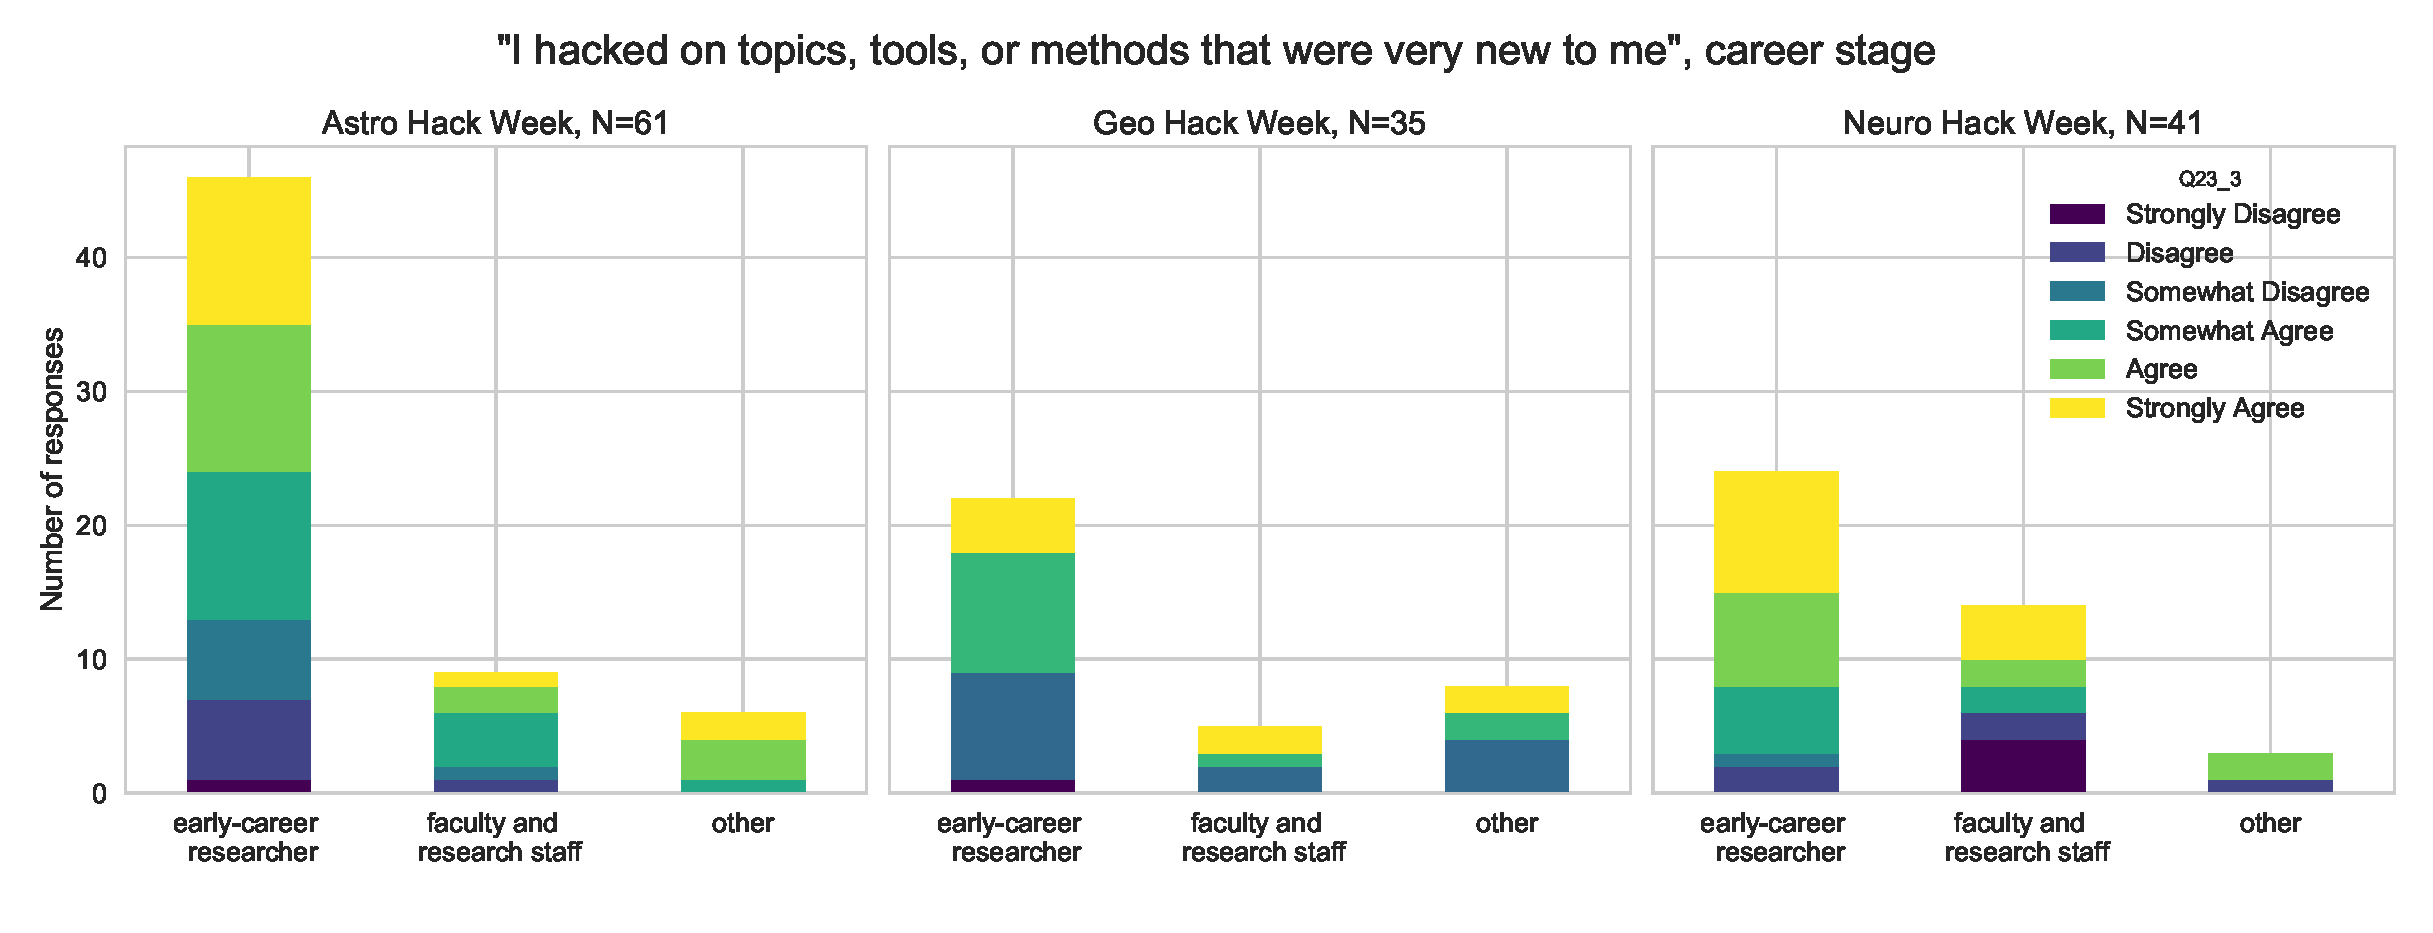
\includegraphics[width=\textwidth]{Q23_3_Q3_stackedbars.eps}
%\end{subfigure}
\caption{}
\label{fig:survey}
%\end{center}
\end{figure*}

\begin{figure*}[h!]
%\begin{center}
%\begin{subfigure}[t]{\textwidth}
\centering
%\caption{}
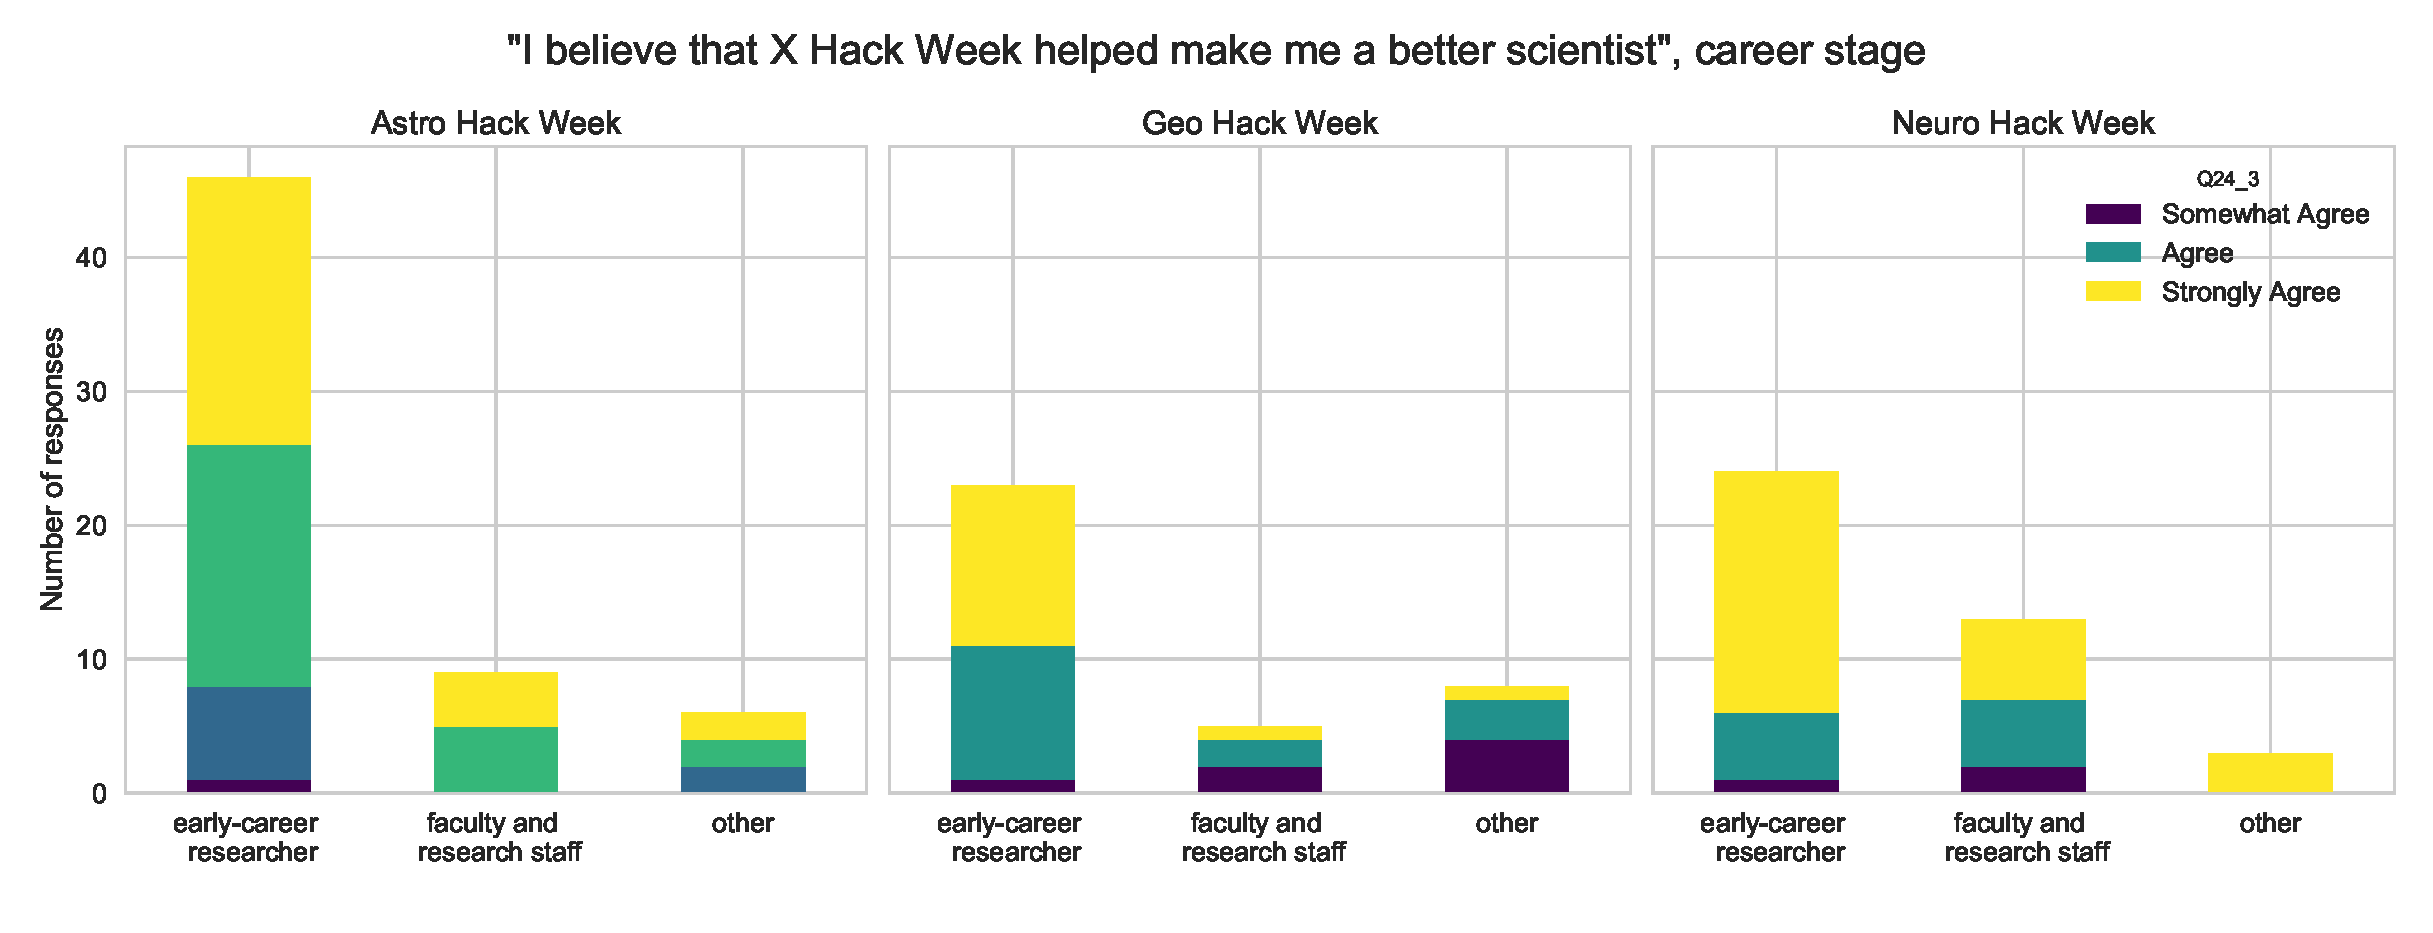
\includegraphics[width=\textwidth]{Q24_3_Q3_stackedbars.eps}
%\end{subfigure}
\caption{}
\label{fig:survey}
%\end{center}
\end{figure*}

\begin{figure*}[h!]
%\begin{center}
%\begin{subfigure}[t]{\textwidth}
\centering
%\caption{}
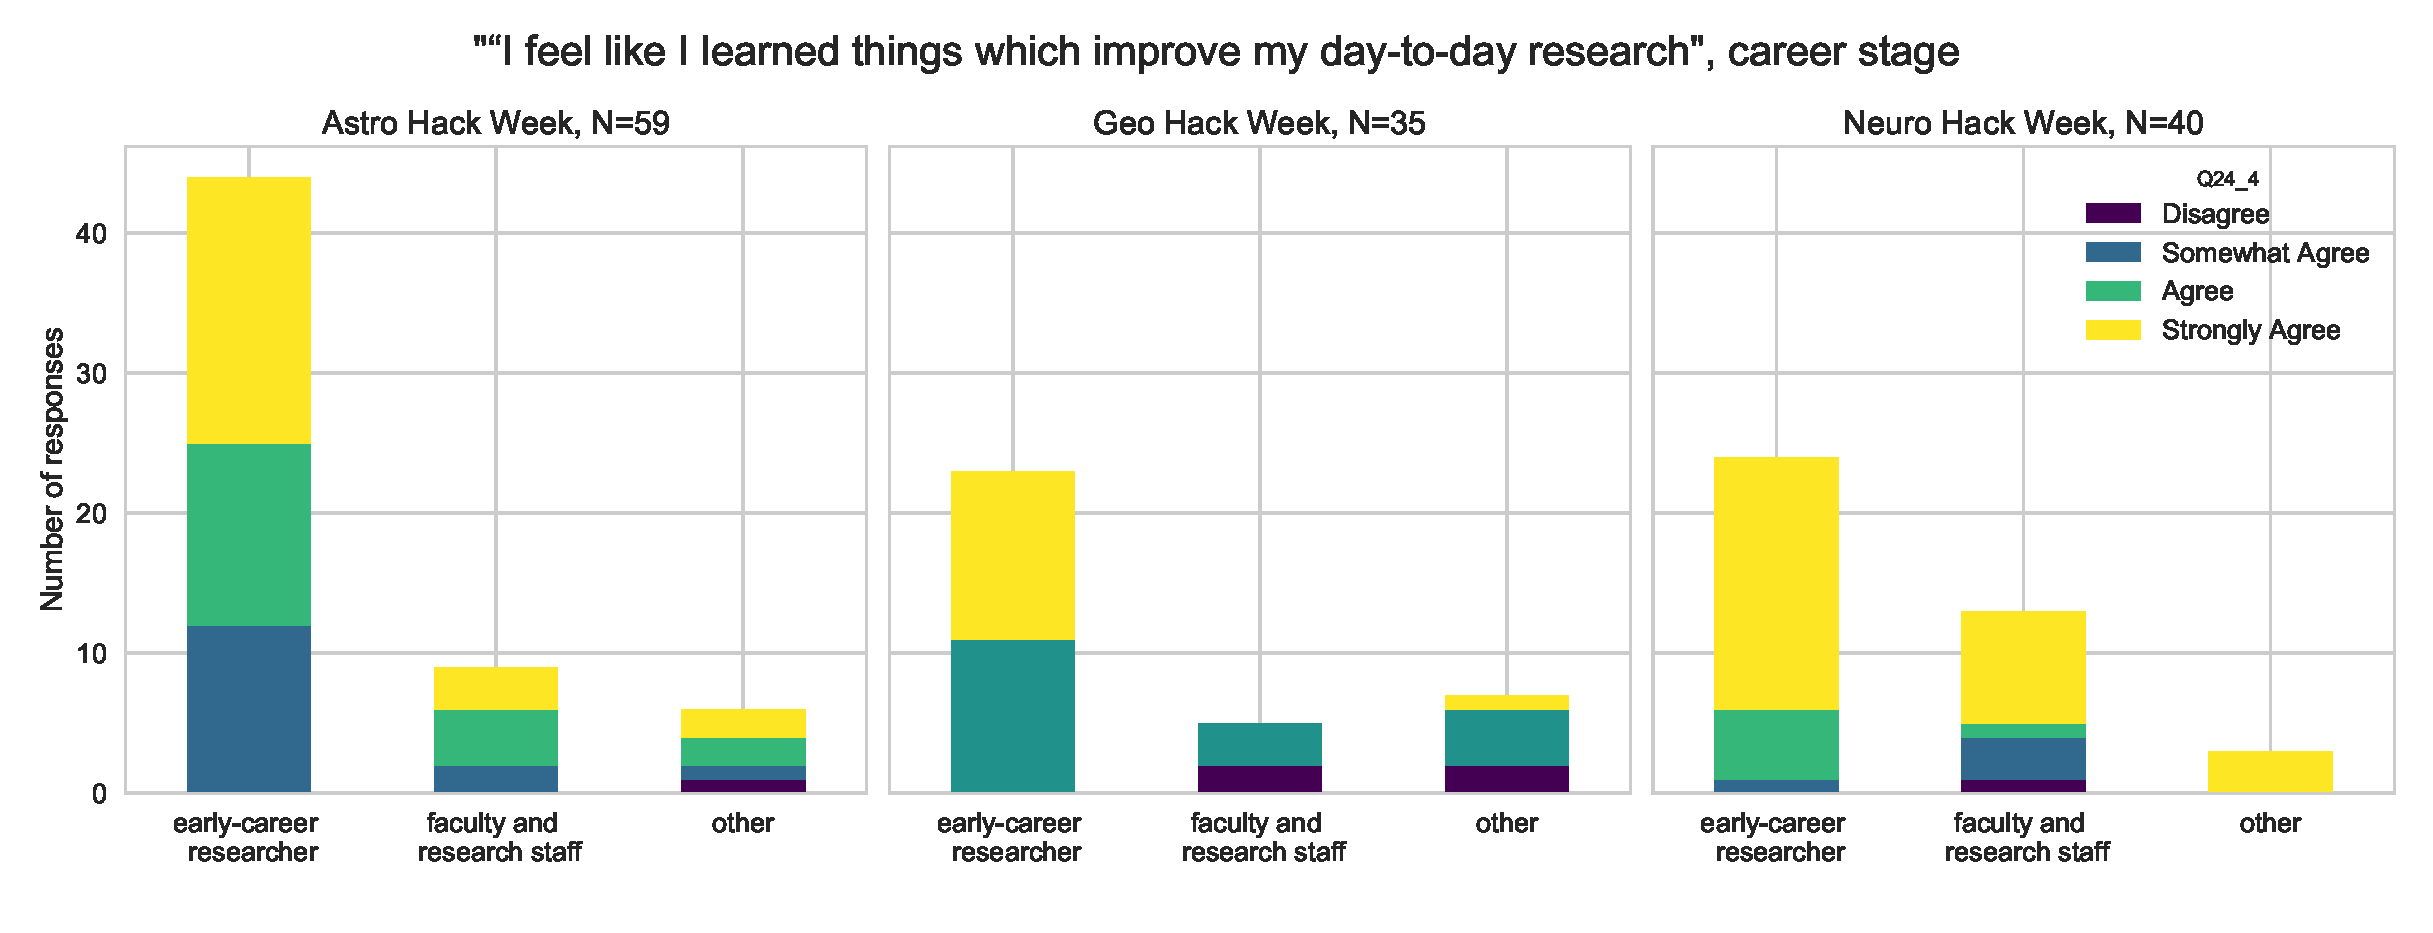
\includegraphics[width=\textwidth]{Q24_4_Q3_stackedbars.eps}
%\end{subfigure}
\caption{}
\label{fig:survey}
%\end{center}
\end{figure*}

\begin{figure*}[h!]
%\begin{center}
%\begin{subfigure}[t]{\textwidth}
\centering
%\caption{}
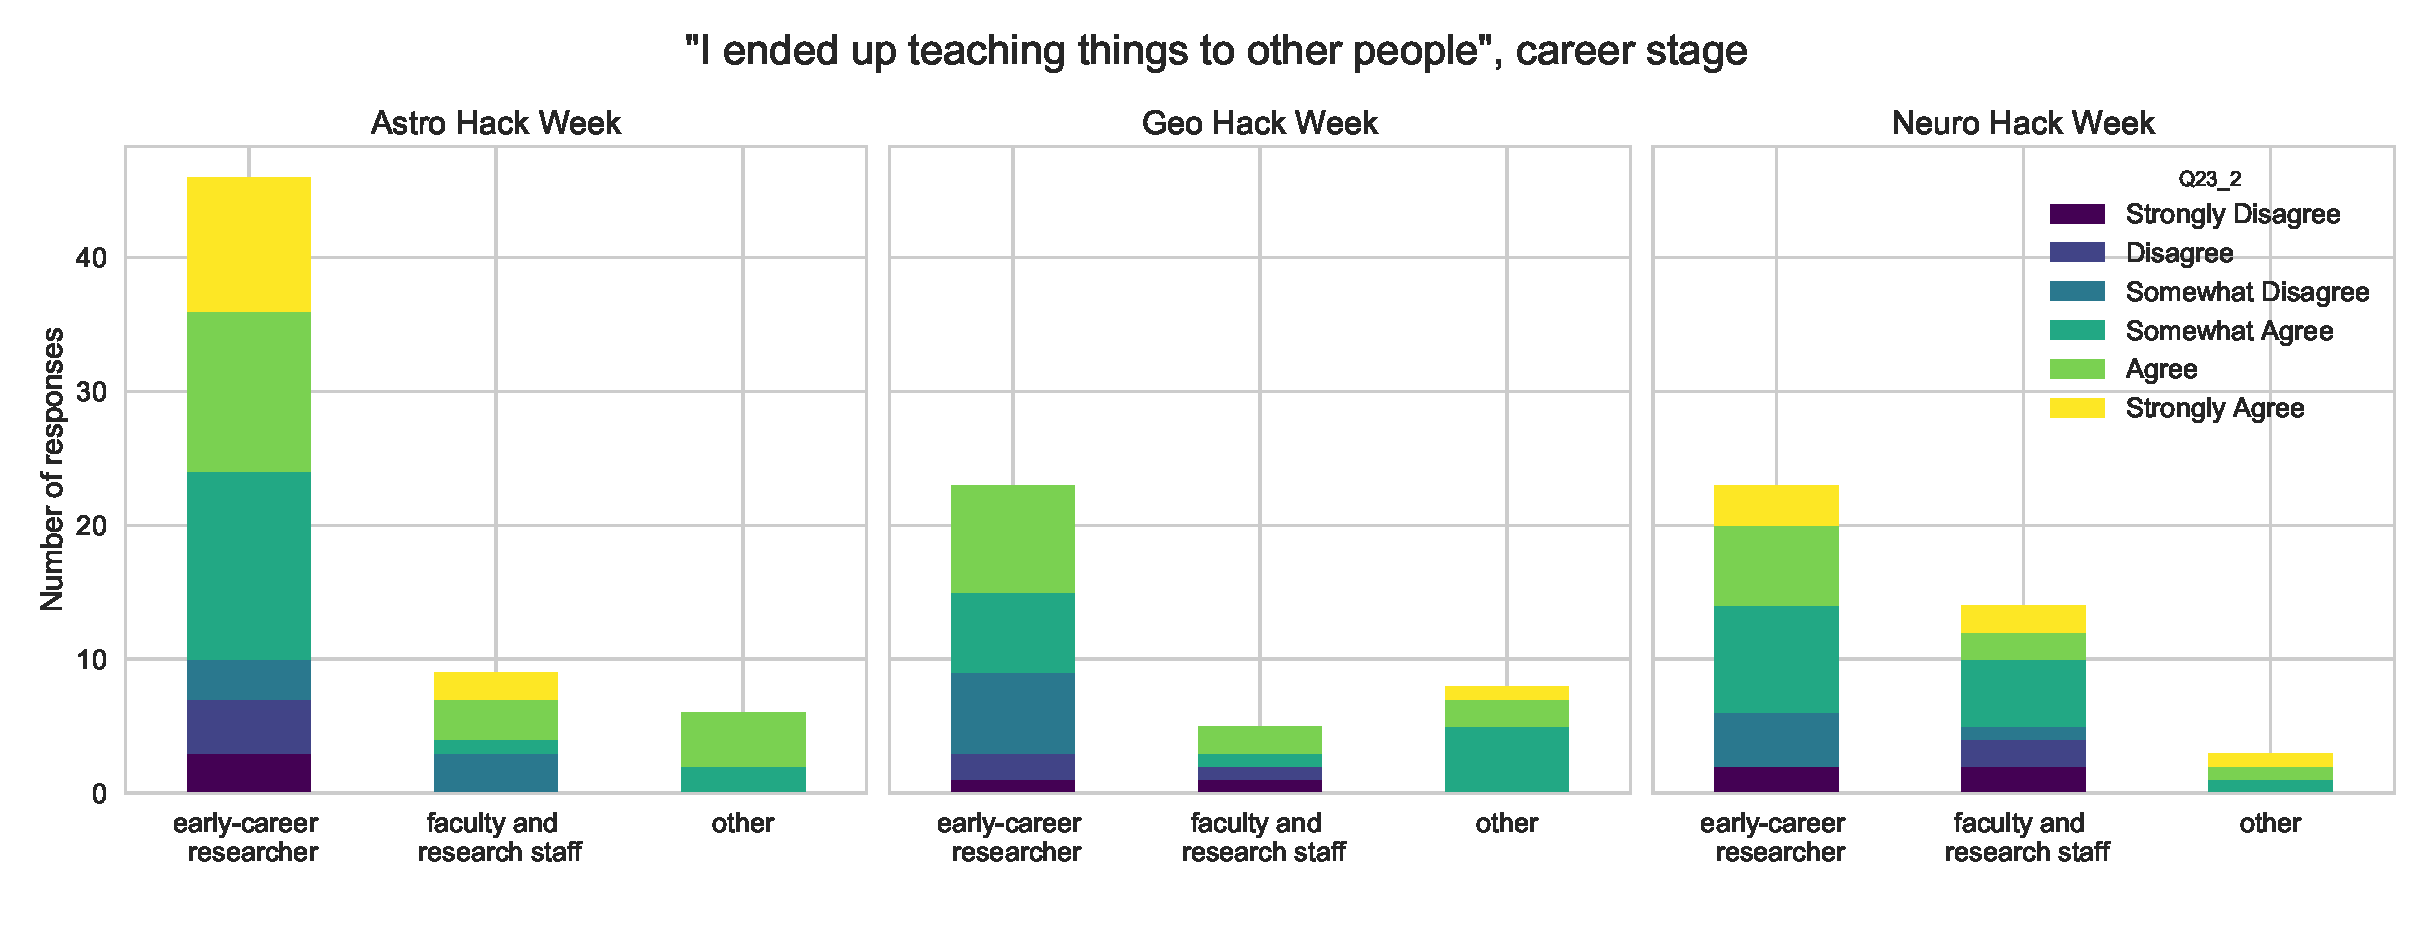
\includegraphics[width=\textwidth]{Q23_2_Q3_stackedbars.eps}
%\end{subfigure}
\caption{}
\label{fig:survey}
%\end{center}
\end{figure*}

\clearpage 

\subsection{Gender Identity}

Here we explore a number of survey responses with gender identity as an independent variable.


\begin{figure*}[h!]
%\begin{center}
%\begin{subfigure}[t]{\textwidth}
\centering
%\caption{}
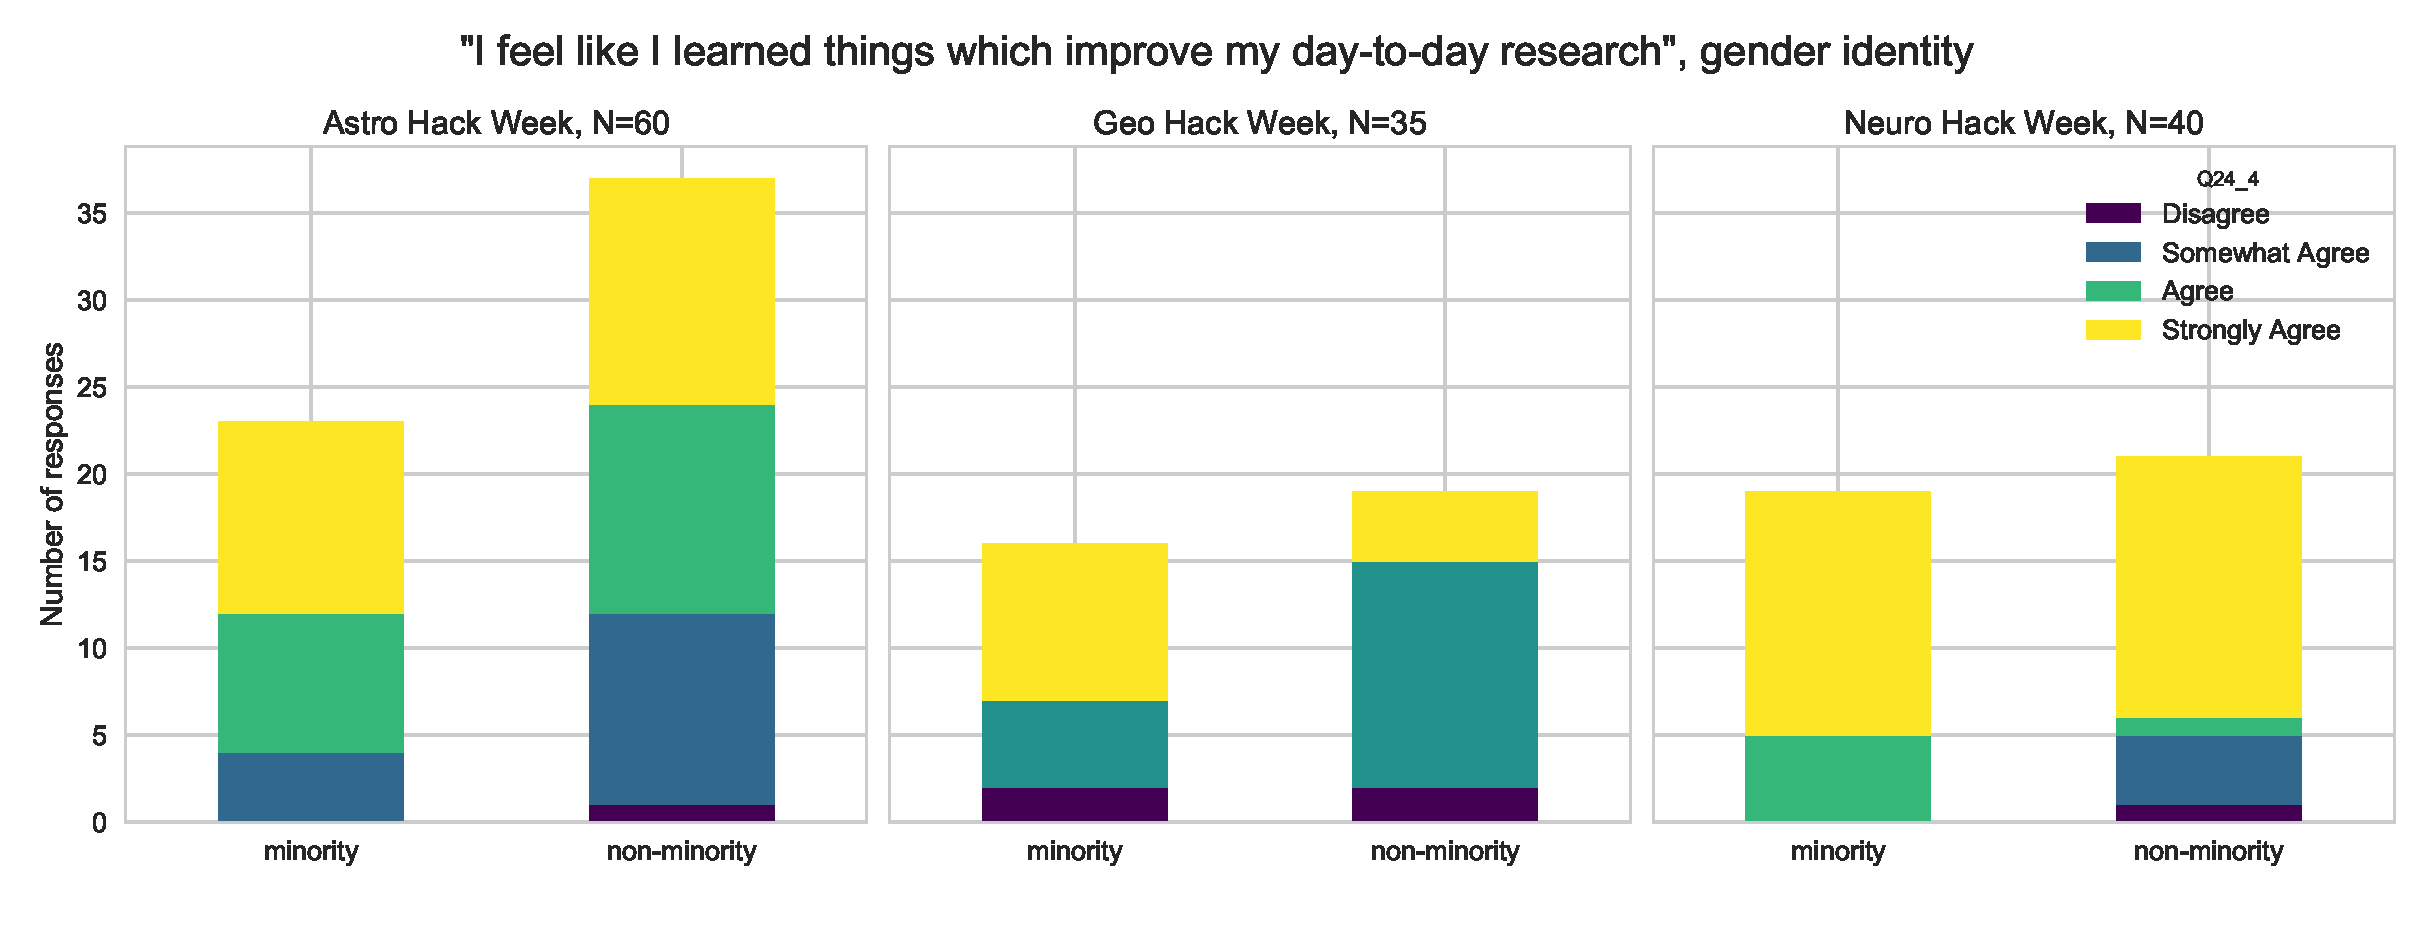
\includegraphics[width=\textwidth]{Q24_4_Q27_stackedbars.eps}
%\end{subfigure}
\caption{}
\label{fig:survey}
%\end{center}
\end{figure*}

\begin{figure*}[h!]
%\begin{center}
%\begin{subfigure}[t]{\textwidth}
\centering
%\caption{}
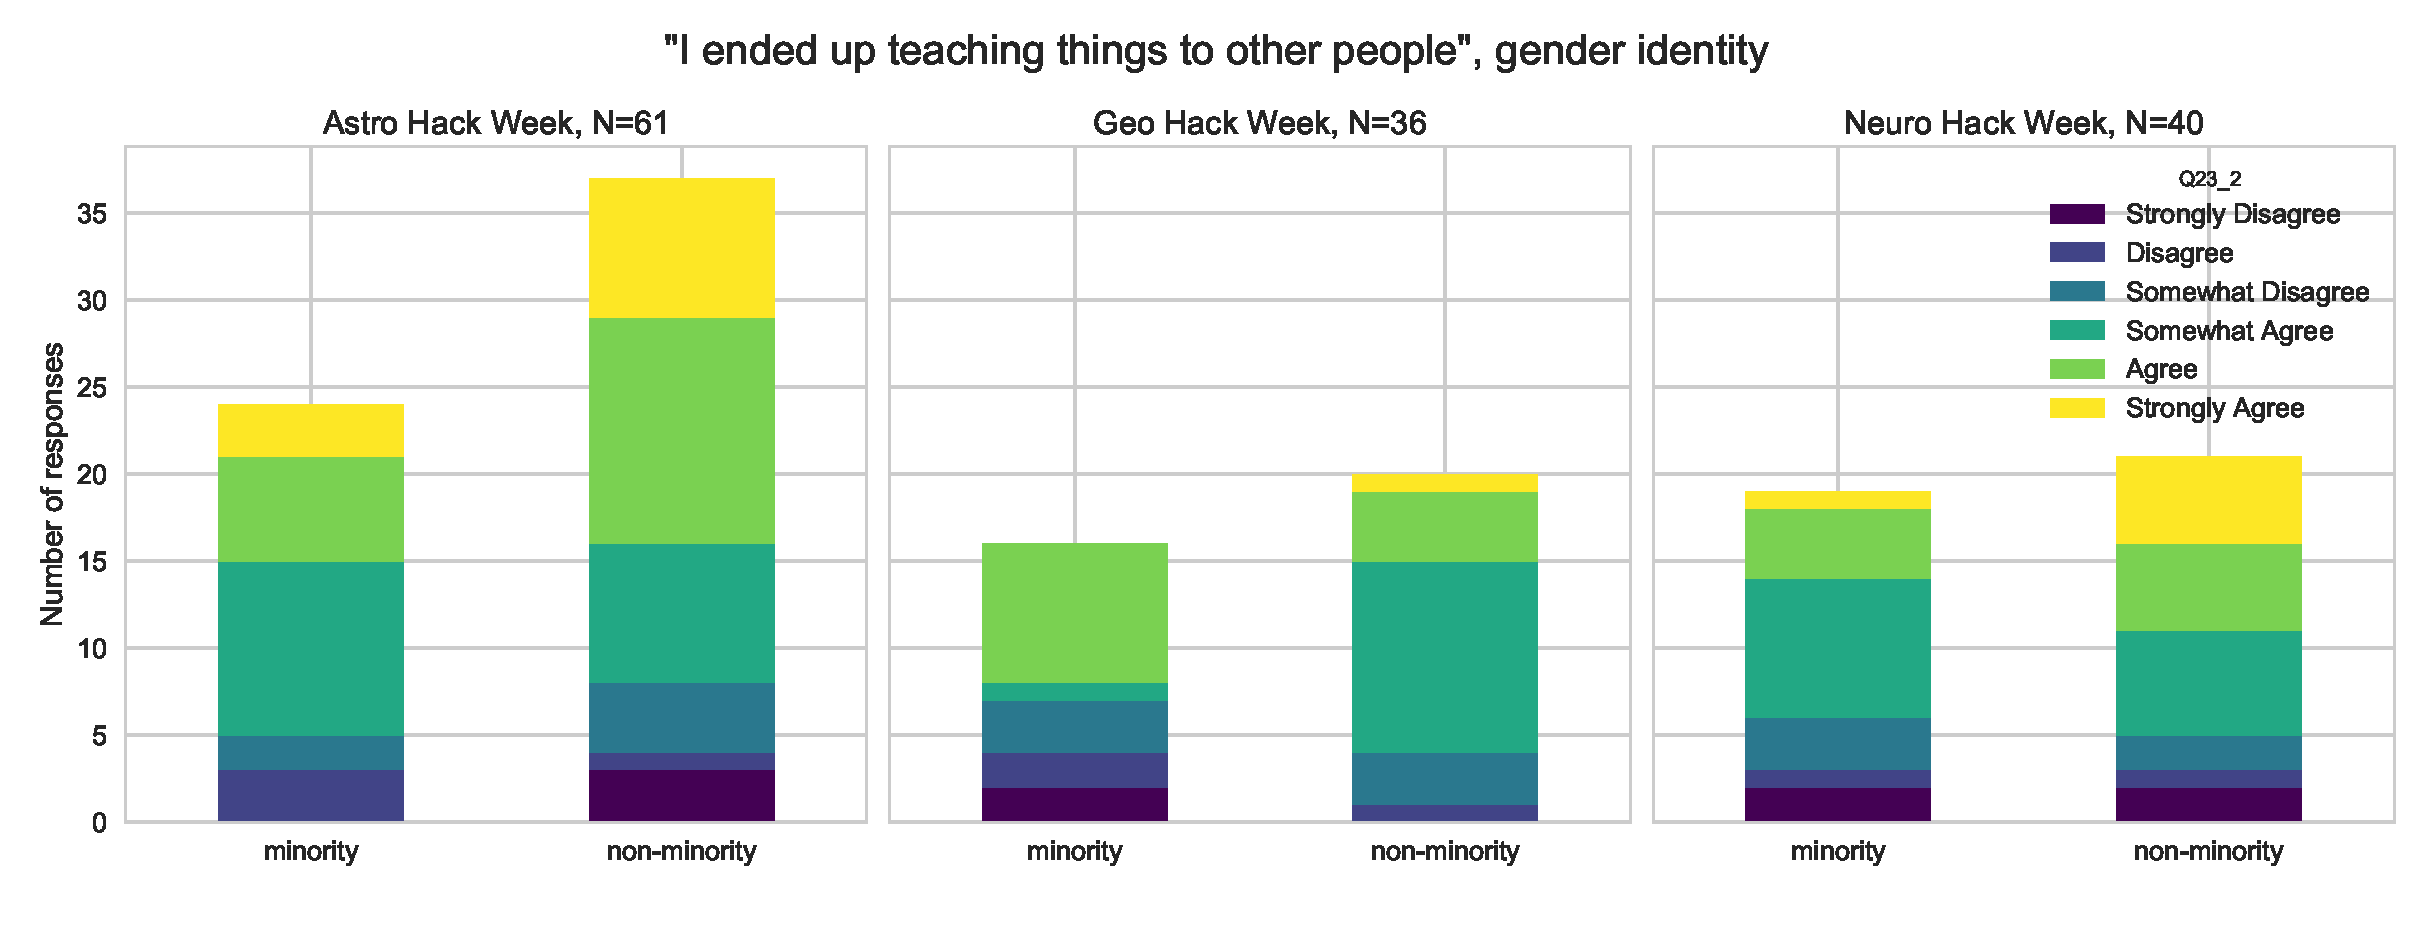
\includegraphics[width=\textwidth]{Q23_2_Q27_stackedbars.eps}
%\end{subfigure}
\caption{}
\label{fig:survey}
%\end{center}
\end{figure*}

\begin{figure*}[h!]
%\begin{center}
%\begin{subfigure}[t]{\textwidth}
\centering
%\caption{}
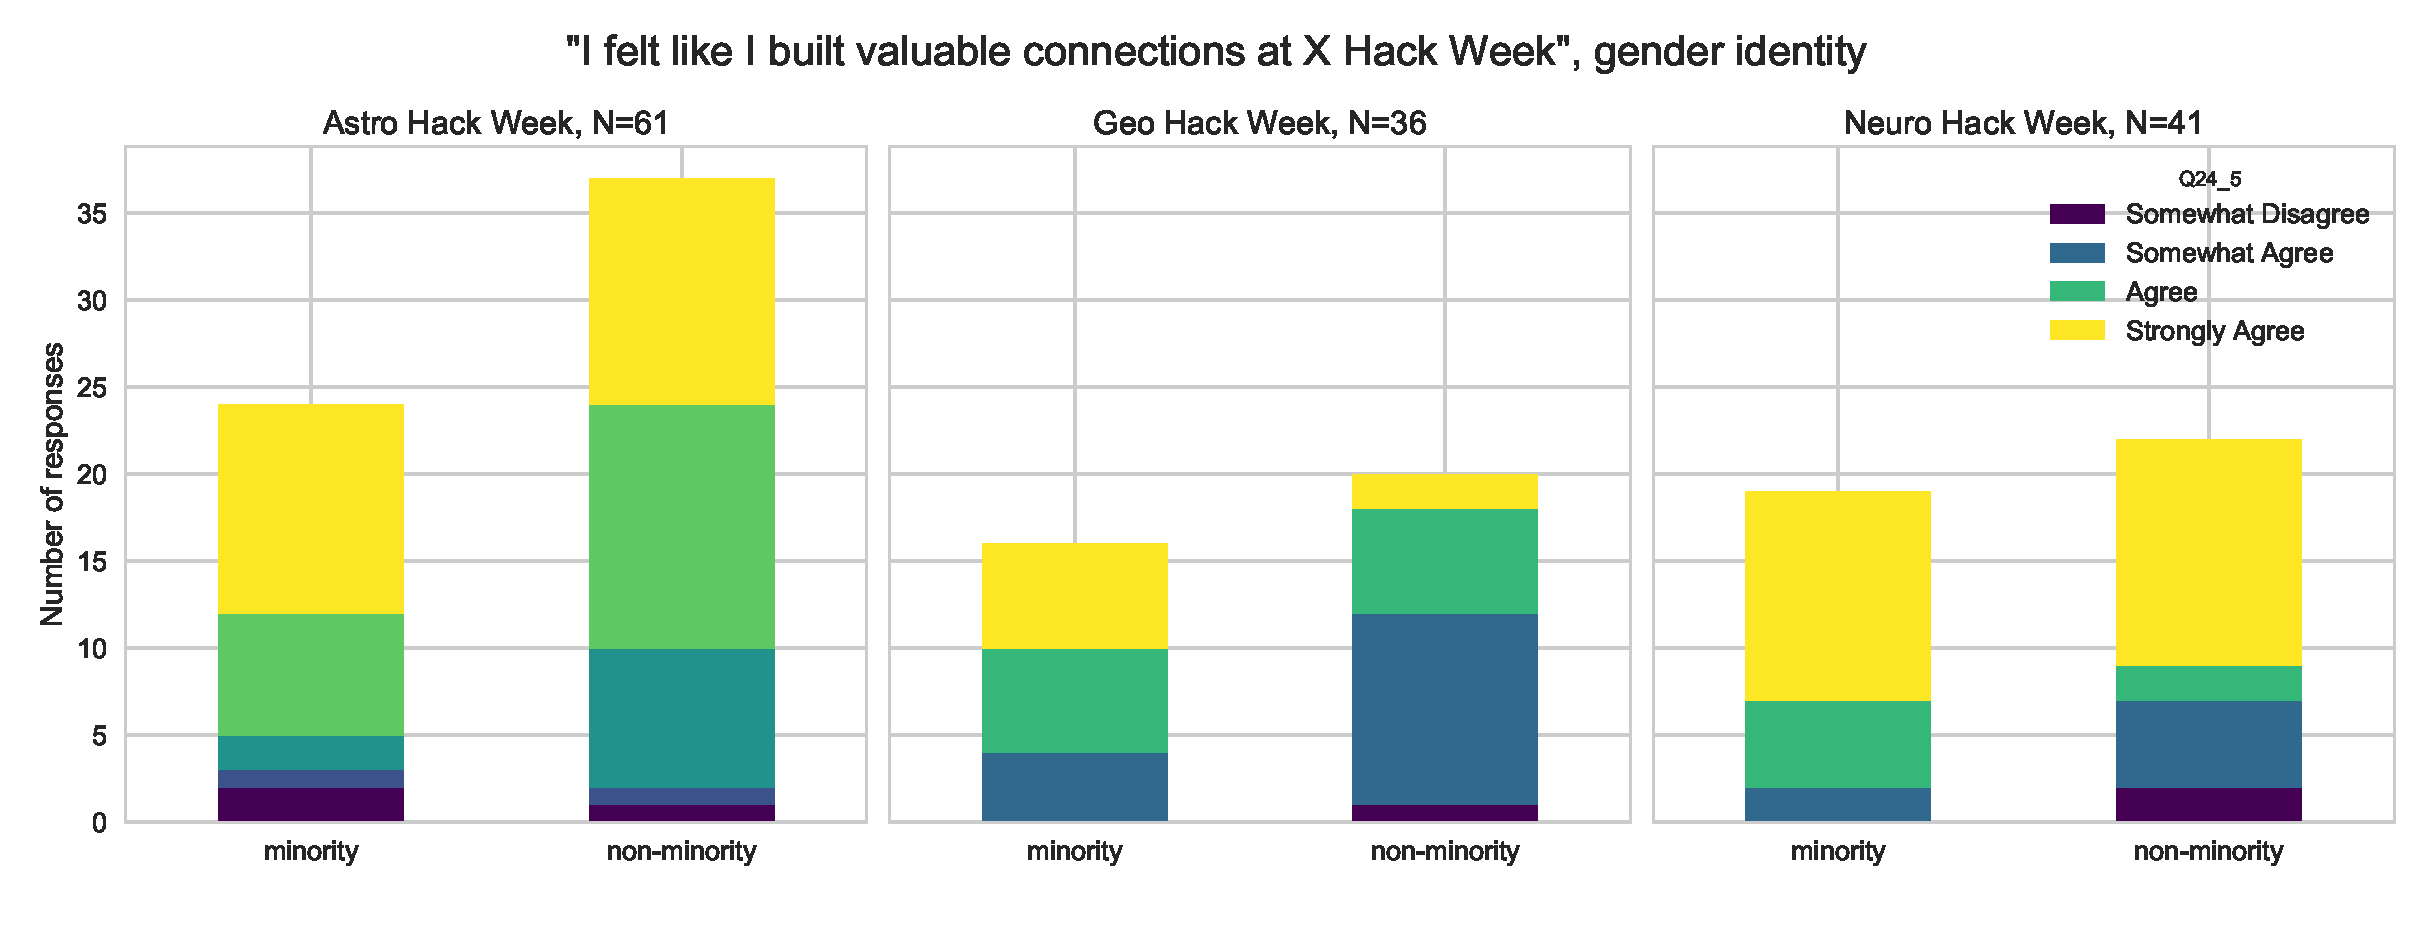
\includegraphics[width=\textwidth]{Q24_5_Q27_stackedbars.eps}
%\end{subfigure}
\caption{}
\label{fig:survey}
%\end{center}
\end{figure*}

\begin{figure*}[h!]
%\begin{center}
%\begin{subfigure}[t]{\textwidth}
\centering
%\caption{}
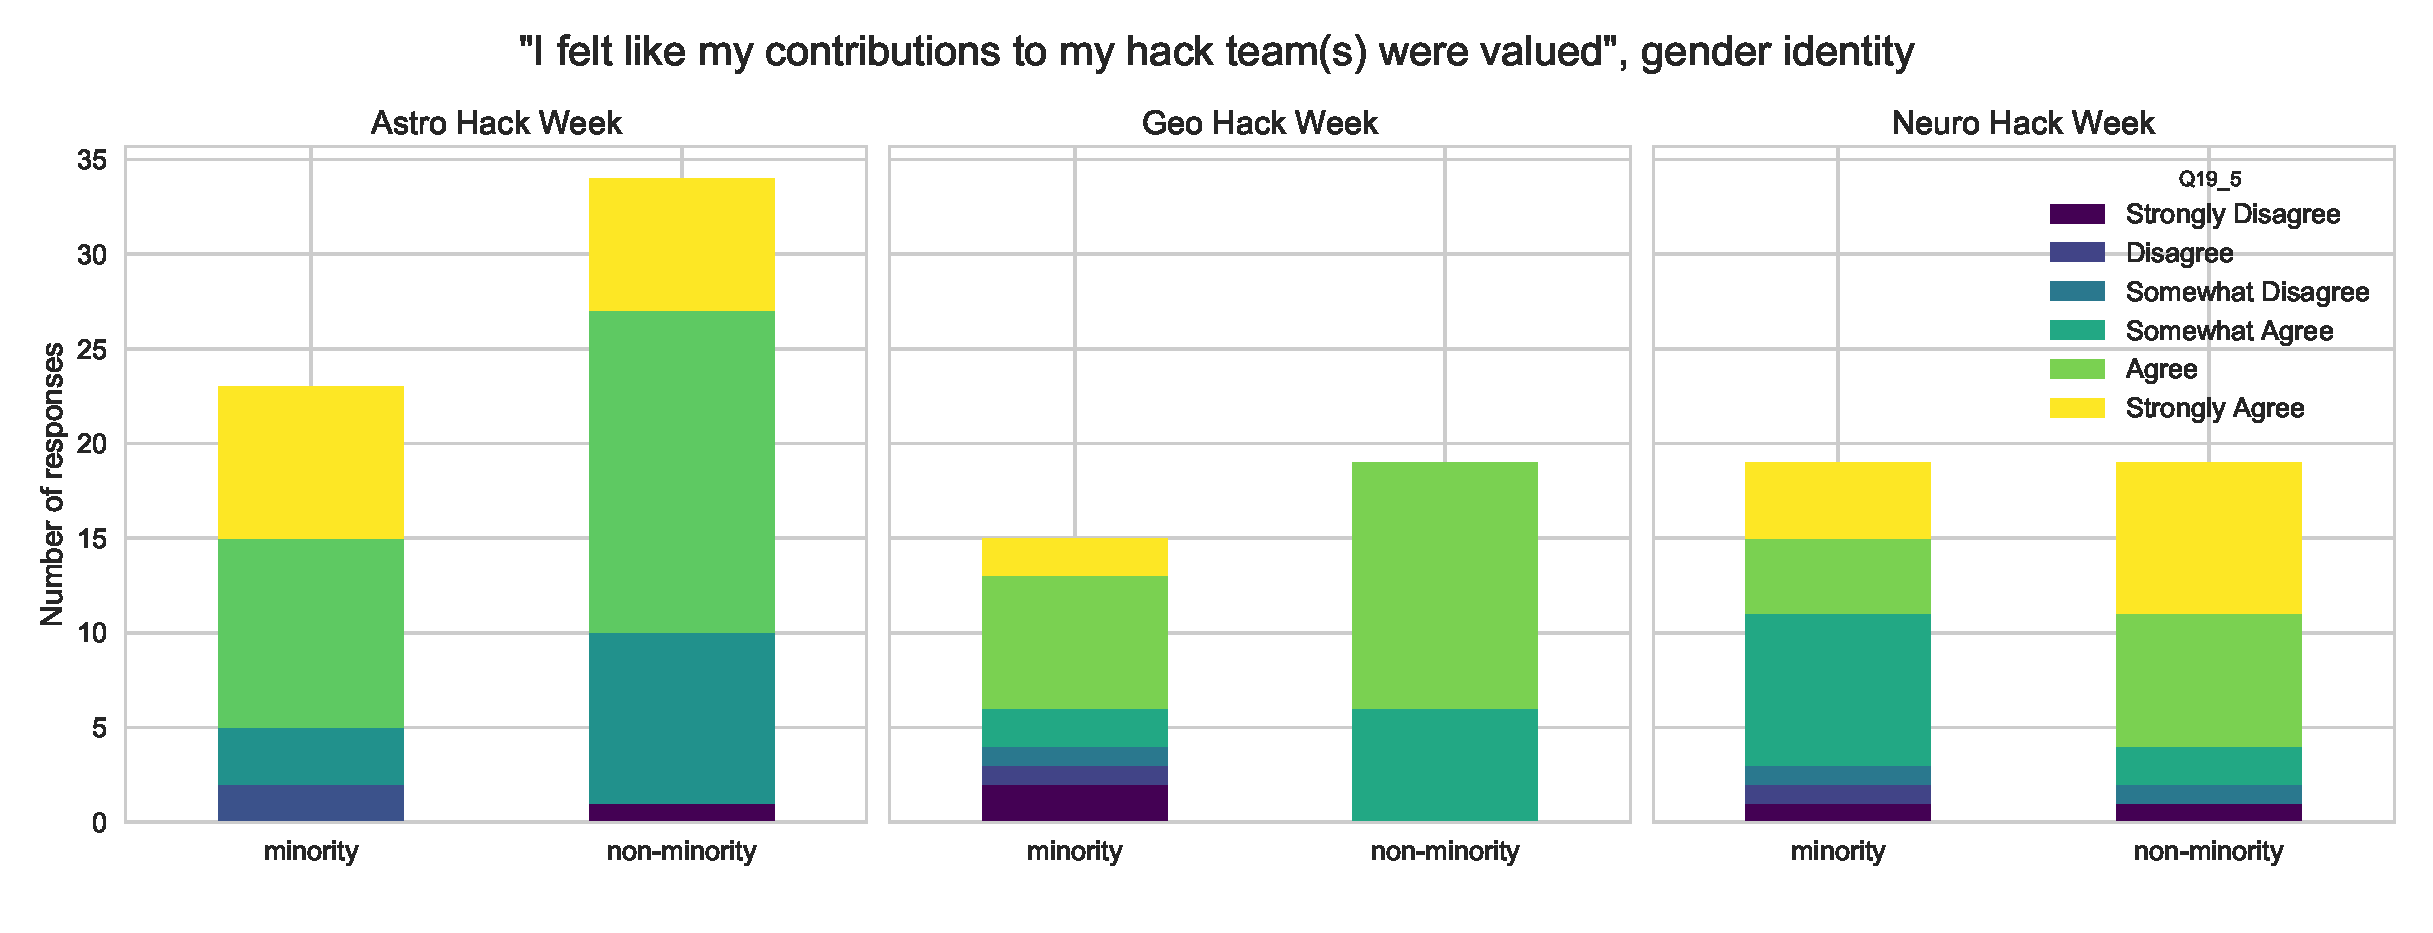
\includegraphics[width=\textwidth]{Q19_5_Q27_stackedbars.eps}
%\end{subfigure}
\caption{}
\label{fig:survey}
%\end{center}
\end{figure*}

\clearpage

\subsection{Racial/Ethnic Identity}

Here we explore a number of survey responses with racial/ethnic identity as an independent variable.

\begin{figure*}[h!]
%\begin{center}
%\begin{subfigure}[t]{\textwidth}
\centering
%\caption{}
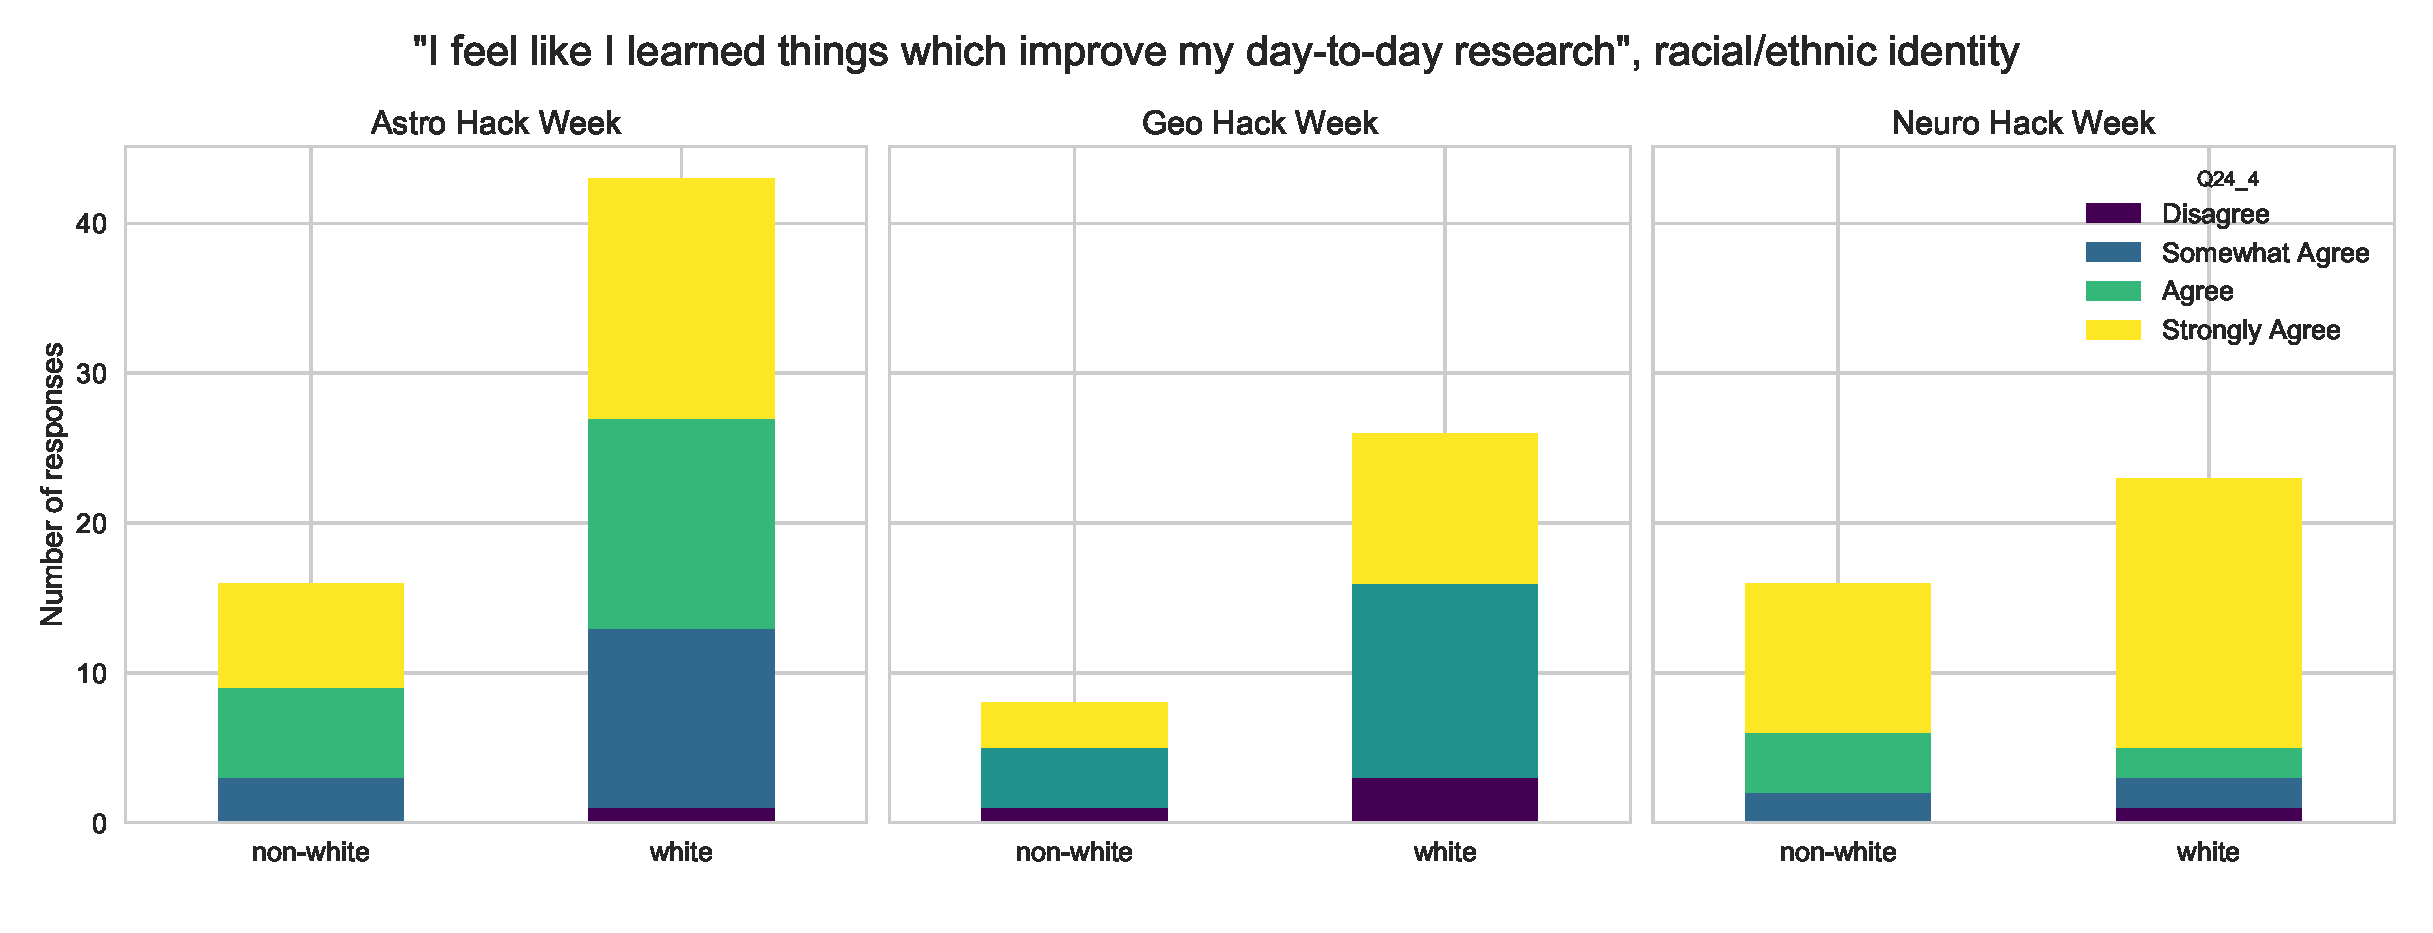
\includegraphics[width=\textwidth]{Q24_4_Q30_stackedbars.eps}
%\end{subfigure}
\caption{}
\label{fig:survey}
%\end{center}
\end{figure*}

\begin{figure*}[h!]
%\begin{center}
%\begin{subfigure}[t]{\textwidth}
\centering
%\caption{}
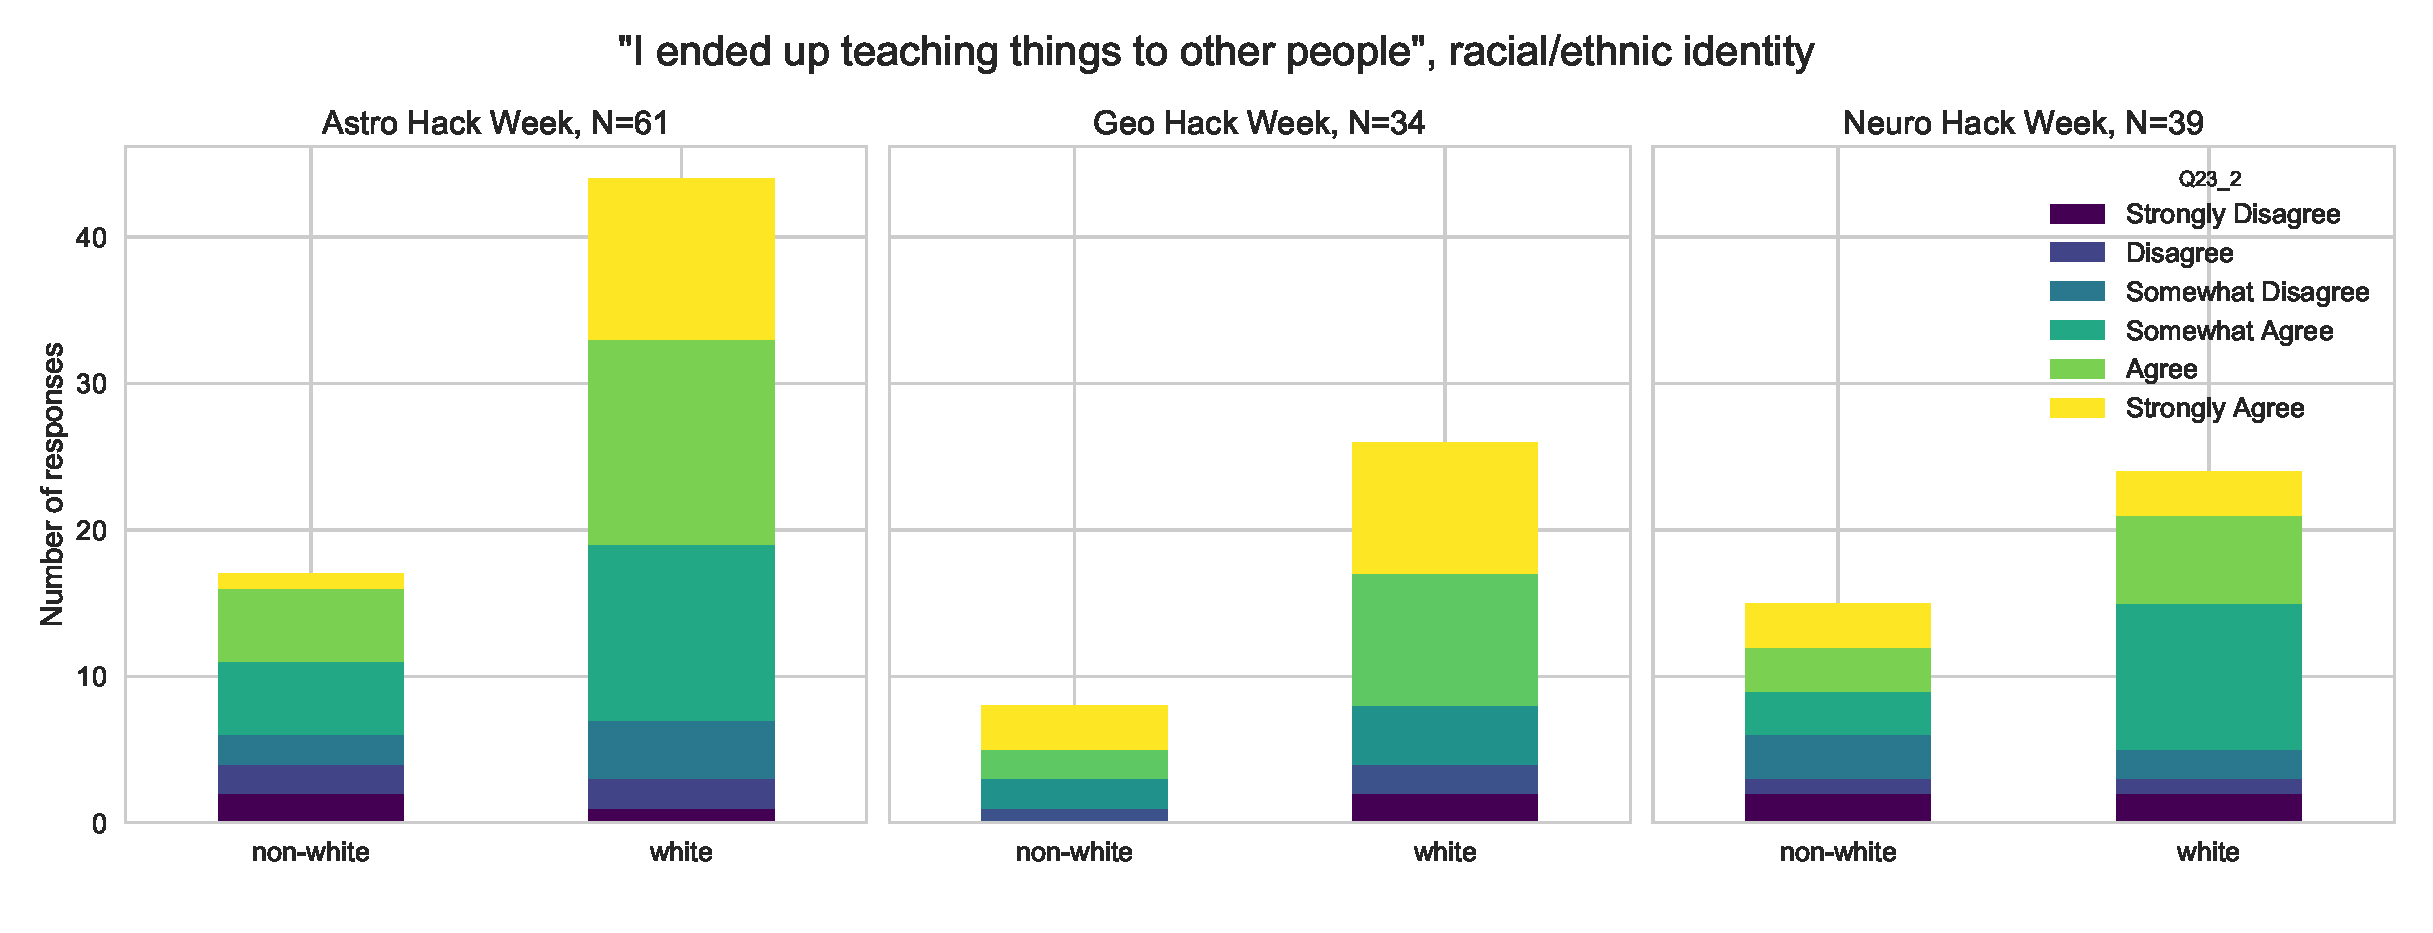
\includegraphics[width=\textwidth]{Q23_2_Q30_stackedbars.eps}
%\end{subfigure}
\caption{}
\label{fig:survey}
%\end{center}
\end{figure*}

\begin{figure*}[h!]
%\begin{center}
%\begin{subfigure}[t]{\textwidth}
\centering
%\caption{}
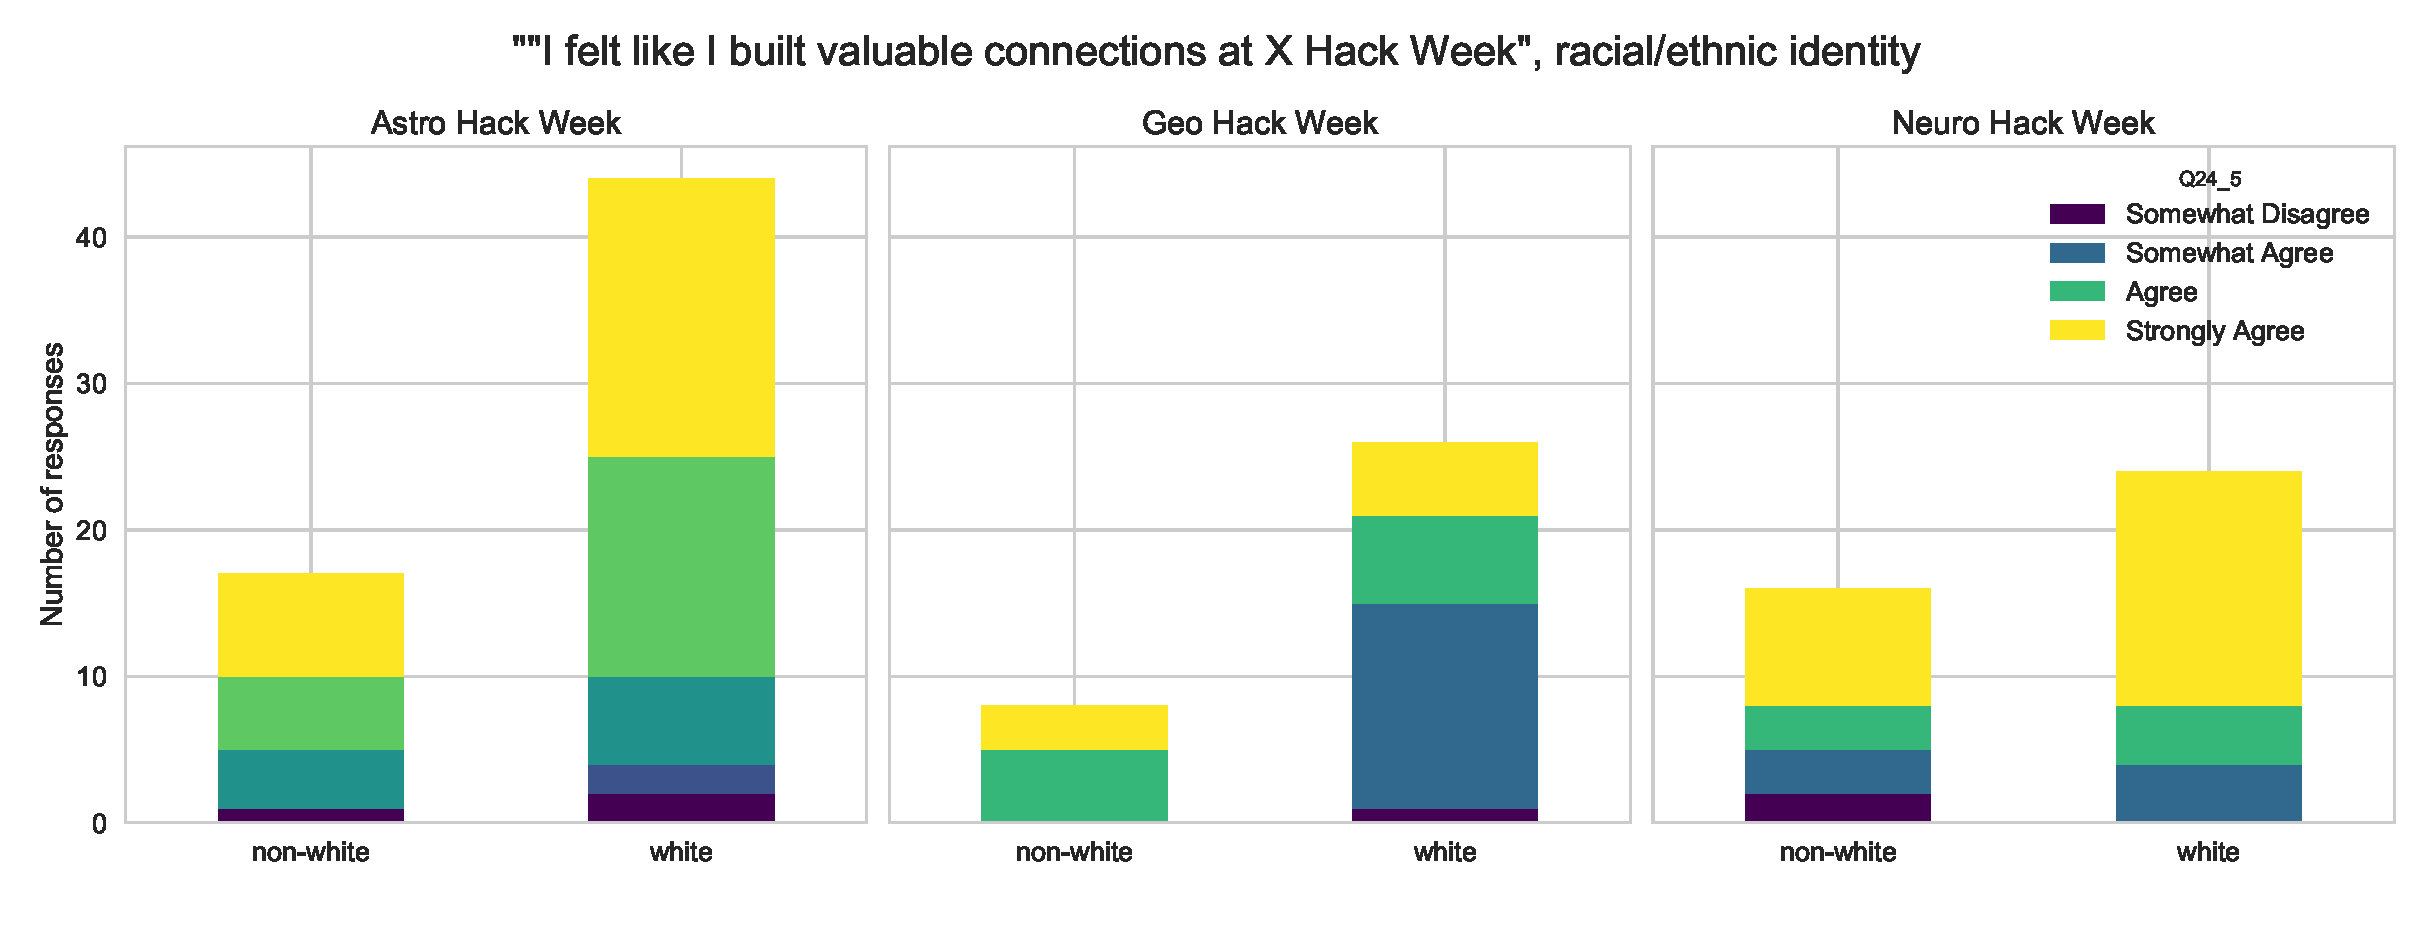
\includegraphics[width=\textwidth]{Q24_5_Q30_stackedbars.eps}
%\end{subfigure}
\caption{}
\label{fig:survey}
%\end{center}
\end{figure*}

\begin{figure*}[h!]
%\begin{center}
%\begin{subfigure}[t]{\textwidth}
\centering
%\caption{}
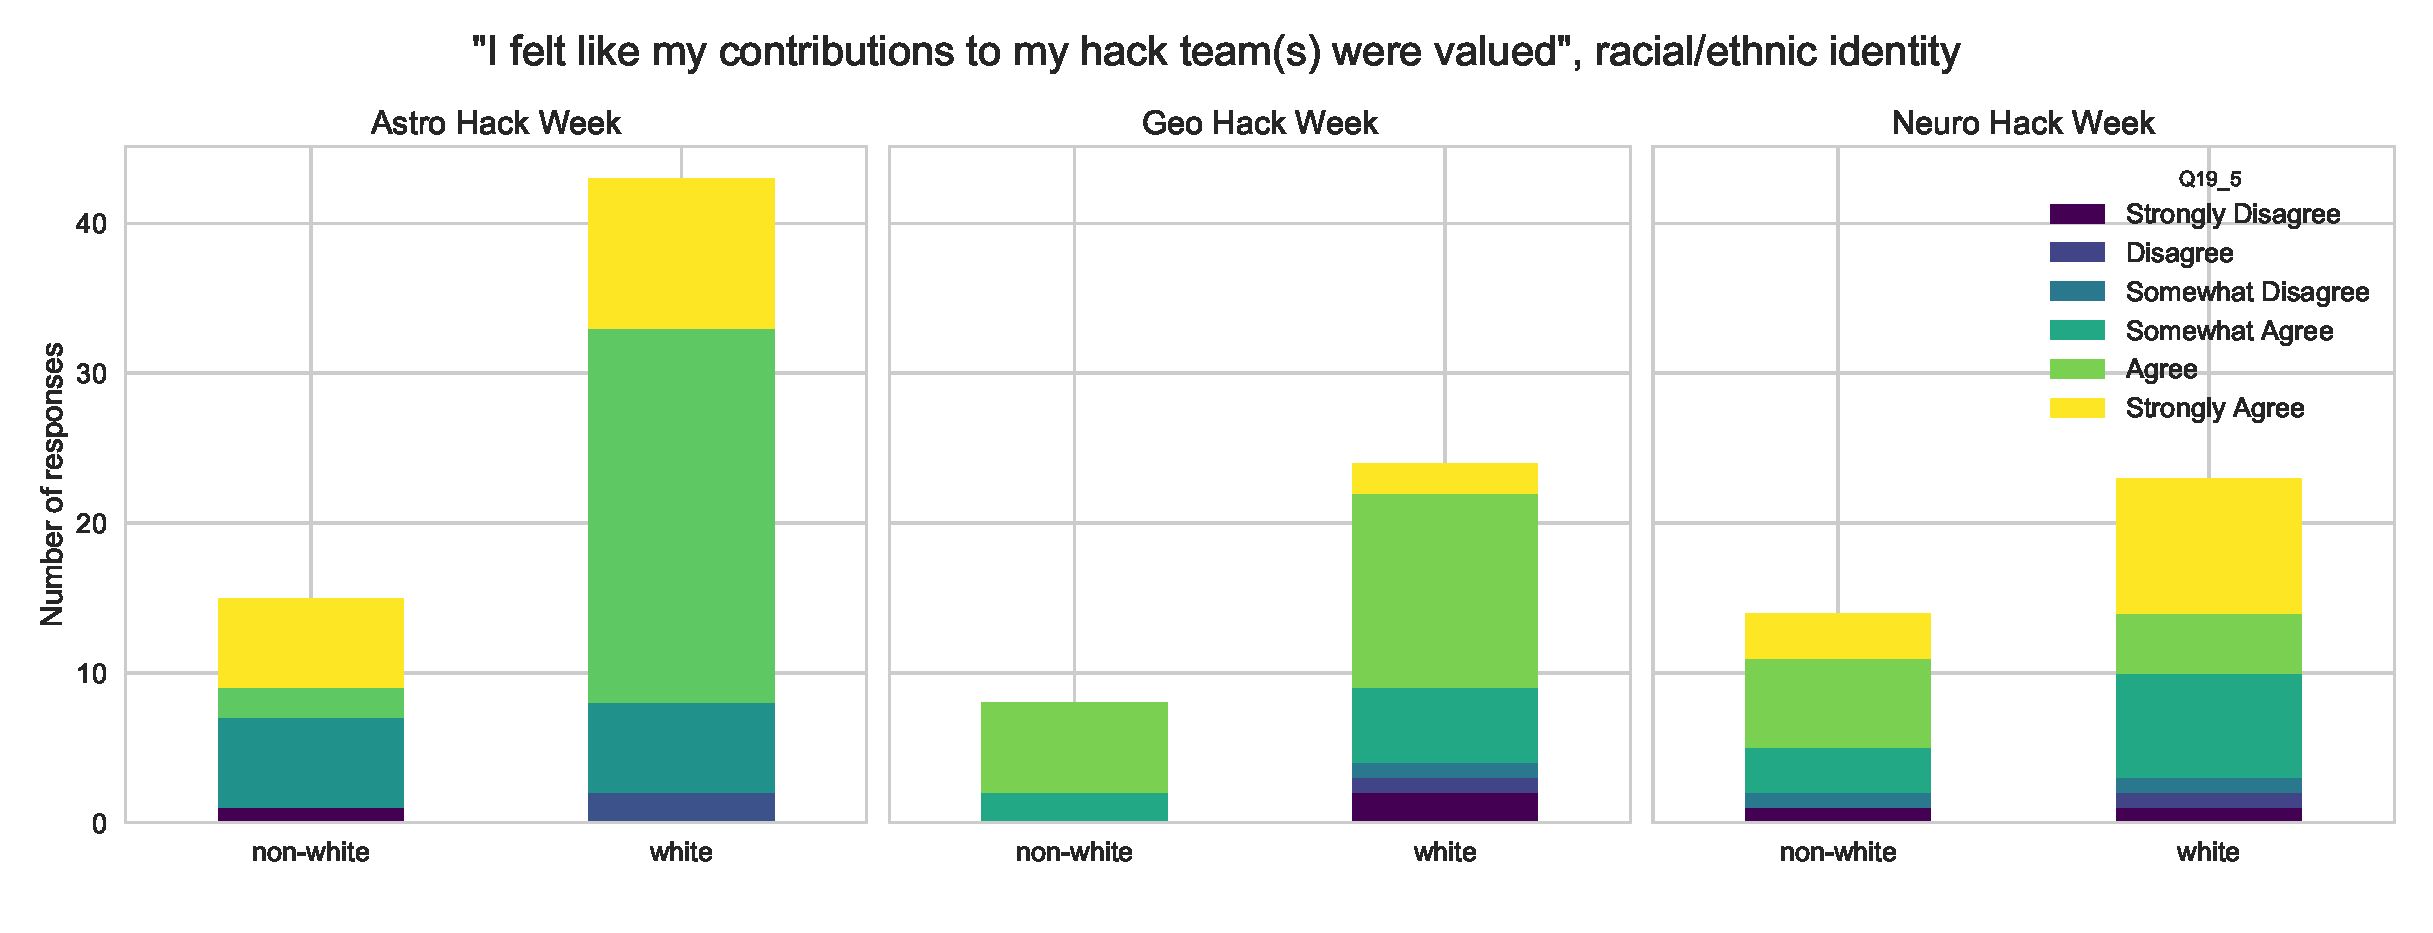
\includegraphics[width=\textwidth]{Q19_5_Q30_stackedbars.eps}
%\end{subfigure}
\caption{}
\label{fig:survey}
%\end{center}
\end{figure*}

\newpage
\bibliographystyle{aasjournal}
\bibliography{paper}

\end{document}
